\documentclass[12pt]{article}
\usepackage[utf8]{inputenc}
\usepackage{xr-hyper}
\usepackage{hyperref}
\usepackage{float}
\usepackage[table,xcdraw]{xcolor}
\usepackage{color, colortbl}
\usepackage{longtable}
\usepackage{booktabs}
\usepackage{graphicx}
\usepackage{multirow}
\usepackage{tikz}
\usepackage{rotating}
\usepackage{caption}
\usepackage{authblk}
\usepackage{csquotes}
\graphicspath{{Figures/}}
\usepackage{setspace}
\usepackage{rotating}
\usepackage{geometry}
\usepackage{array}
\usepackage{lscape}
\usepackage{longtable}
\usepackage{etoolbox}
\usepackage{hhline}
\usepackage{lmodern}
\usepackage[
backend = biber,
natbib,
citestyle = authoryear,
bibstyle = apa,
maxcitenames = 2, 
maxbibnames = 99, 
uniquename=false,
uniquelist=false
%sorting = none % sort by name year title
]{biblatex}
\addbibresource{Ref_invertebrate_DB.bib}

\usepackage{subfiles} % Best loaded last in the preamble

%%%% Functions and definitions %%%%%%%%%%%%%%%%%%%%%%%%%%%%%%
\definecolor{Gray}{gray}{0.9}

% horizontal space between two columns
\setlength{\tabcolsep}{2mm}

%%%%% New Commands %%%%%%%%%%%%%%%%%%%%%%%%%%%%%%%%%%%%%%%%%%

\makeatletter
\newcommand*{\addFileDependency}[1]{% argument=file name and extension
  \typeout{(#1)}
  \@addtofilelist{#1}
  \IfFileExists{#1}{}{\typeout{No file #1.}}
}
\makeatother

\newcommand*{\myexternaldocument}[1]{%
    \externaldocument{#1}%
    \addFileDependency{#1.tex}%
    \addFileDependency{#1.aux}%
}

\newcommand{\specialcell}[2][c]{%
  \begin{tabular}[#1]{@{}c@{}}#2\end{tabular}}

\renewcommand*{\thefootnote}{\alph{footnote}}

% raplace "and" in authoryear in-text citations with "&" 
\renewcommand*{\finalnamedelim}{%
  \ifnumgreater{\value{liststop}}{2}{\finalandcomma}{}%
  \addspace\&\space}

% Keywords command
\providecommand{\keywords}[1]
{
  {\small	
  \textbf{\textit{Keywords---}} #1
}}

%%%% Formatting options %%%%%%%%%%%%%%%%%%%%%%%%%%%%%%%%%%%%%
\onehalfspacing

\listfiles

\myexternaldocument{Latex_Supplementary_File}

%%%%%%%%%%%%%%%%%%%%%%%%%%%%%%%%%%%%%%%%%%%%%%%%%%%%%%%%%%%%%%%%%%%%%%%%%%%%%%%%%%
%%%%%%%%%%%%%%%%%%%%%%%%%%%%%%%%%%%%%%%%%%%%%%%%%%%%%%%%%%%%%%%%%%%%%%%%%%%%%%%%%%
\title{Tackling discrepancies in freshwater invertebrate trait databases: Harmonising across continents and aggregating taxonomic resolution}
\author[1]{Stefan Kunz}
\author[2]{Ben J. Kefford}
\author[3]{Astrid Schmidt-Kloiber}
\author[4]{Christoph D. Matthaei}
\author[5]{Philippe Usseglio-Polatera}
\author[3]{Wolfram Graf}
\author[6]{N. LeRoy Poff}
\author[7]{Leon Metzeling}
\author[8]{Laura Twardochleb}
\author[9]{Charles P. Hawkins}
\author[1]{Ralf B. Schäfer}
\affil[1]{Institute for Environmental Sciences, University of Koblenz-Landau, Landau, Germany}
\affil[2]{Centre for Applied Water Science, Institute for Applied Ecology, University of Canberra, Canberra, Australia}
\affil[3]{Institute of Hydrobiology and Aquatic Ecosystem Management, University of Natural Resources and Life Sciences Vienna (BOKU), Vienna, Austria}
\affil[4]{Department of Zoology, University of Otago, Dunedin, New Zealand}
\affil[5]{University of Lorraine, CNRS, LIEC, Metz, France}
\affil[6]{Department of Biology, Colorado State University, Fort Collins, USA}
\affil[7]{Environment Protection Authority Victoria, Applied Sciences Division, Macleod, Australia}
\affil[8]{Department of Fisheries and Wildlife, Michigan State University, East Lansing, USA}
\affil[9]{Department of Watershed Sciences, National Aquatic Monitoring Center, and the Ecology Center, Utah State University, Logan, USA}
\date{}

\begin{document}
\maketitle

\newpage

\section*{Abstract}

1. Use of invertebrate traits rather than species composition may facilitate large-scale comparisons of community structure and responses to disturbance in freshwater ecology because the same traits can potentially occur everywhere.  In recent years, comprehensive invertebrate trait databases have been established at different scales (e.g. regions, continents). The wide availability of invertebrate trait data supports trait-based studies, especially at large scales. However, a number of data-related issues complicate the use of invertebrate traits for ecological studies. For example, standardised definitions for freshwater invertebrate traits are lacking, which impedes comparisons across regions. Moreover, it is uncertain how harmonising varying trait definitions among databases might influence identification of trait-environment relationships. In addition, taxonomic resolution between taxonomic composition data and trait data can differ, making aggregation of traits necessary. At present, it is unknown how different trait aggregation approaches compare with expert-assigned trait affinities. In this study we aimed to identify discrepancies in trait definitions across freshwater invertebrate databases and to compare trait aggregation methods to identify how phylogenetic structure and trait variability influence results from different aggregation methods.

2. We describe discrepancies in the definitions of traits used to create freshwater invertebrate trait databases in Europe, North America, New Zealand, and Australia. Based on our comparisons of these trait databases, we established four novel trait datasets by harmonising trait definitions of commonly used traits. Next, we used two of these datasets to compare aggregated traits obtained by different aggregation methods with traits assigned by experts, both at the family level. The trait aggregation methods we compared used either the mean or the median and different weightings. We further explored the effects of harmonisation and trait aggregation by re-analysing data from a case study.

3. We found that among trait databases, trait definitions often differed because varying numbers of traits were used to describe groups of related traits (e.g., respiration traits) and the focus of descriptions for groups of related traits also varied (e.g., for feeding mode some databases focused on the food source, whereas others focused on mouthpart morphology). The coding to describe traits (binary, fuzzy) also varied among databases. Our comparison of different aggregation methods showed that family-level aggregated and expert-assigned traits were similar, especially when aggregation was based on the median, and that trait coding method, uneven phylogenetic structure, and high trait variability can influence aggregated trait affinities. We further showed that harmonised and aggregated data performed similarly to not aggregated and harmonised data from the case study in identifying trait–environment relationships.

4. By identifying discrepancies in trait definitions we hope to motivate the development of standardised terminology for invertebrate traits. Our results also illustrate the usefulness of harmonised datasets for ecological study and provide guidance for the circumstances under which the choice of trait aggregation method is important.
\\
\keywords{trait definitions, trait aggregation, data synthesis, trait-environment relationships, large-scale comparisons}


\newpage

\section*{Introduction}

Explaining and predicting how communities are shaped by environmental factors is a primary goal of ecology. Species traits are measurable properties of an organism (\cite{mcgill_rebuilding_2006}), and comparing communities based on the traits possessed by species may facilitate testing of a range of ecological hypotheses (\cite{statzner_perspectives_2001}). Traits are assumed to be adaptations (e.g., physiological, behavioural) of organisms to their environment, which represent either direct or indirect linkages between the biological response of an organism or a population and its environment (\cite{southwood_habitat_1977, verberk_delivering_2013}). In addition to providing local-scale mechanistic-based expressions of species-environment relationships, trait-based approaches might be suitable for large-scale analyses of environmental risks to communities because the occurrence and distribution of traits are less constrained by biogeographic boundaries than that of taxa (\cite{baird_toward_2011, bonada_taxonomic_2007}). 

Invertebrate traits have been increasingly used in freshwater ecology, e.g. by relating macroinvertebrate trait composition to environmental factors such as climate change or salinisation (\cite{bhowmik_large_2015, poff_developing_2010, szocs_effects_2014}), for predicting changes in ecosystem functioning and trophic dynamics (\cite{vos_taxonomic_2017, gutierrez-canovasPopulationsHighvaluePredators2021}), or for developing indices for biomonitoring (\cite{beketov_spear_2009}). In the last decades, freshwater ecologists have compiled comprehensive invertebrate trait databases, which typically include data for a single region or continent (\cite{kefford_integrated_2020, Philips_and_Smith_NZ_DB_2018, schmidt-kloiber_www.freshwaterecology.info_2015, tomanova_trophic_2006, ussegliopolatera_biological_2000, vieira_database_nodate, gayraudInvertebrateTraitsBiomonitoring2003, statznerConservationTaxonomicBiological2007}). The availability of invertebrate trait data from different continents enables comparisons of regional trait variation and allows for testing the consistency of trait structure–environmental factor relationships across both small and large spatial extents. To date, such analyses have been carried out mostly within continents, using information from one or two trait databases. For example, \citet{bonada_taxonomic_2007} compared trait composition for Mediterranean and temperate regions in Europe based on traits from \citet{ussegliopolatera_biological_2000} (typically referred to as the Tachet database), \citet{poff_developing_2010} characterised trait composition across sites in the Western USA based on traits from \citet{poff_functional_2006}, and \citet{botwe_effects_2018} used trait definitions from \citet{poff_functional_2006} and \citet{schafer_trait_2011} to test for effects of salinity on invertebrate traits across different sites in South Australia. Analyses that synthesise invertebrate trait information from more than two different continents are rare, but see \citet{brown_functional_2018} and \citet{statzner_reproductive_1997}. 

The variability and inconsistencies of information in freshwater invertebrate trait databases, besides the diversity of taxa across regions, is likely a major reason for the lack of comparisons across continents. Several challenges currently prevent the use of invertebrate trait data from different established databases in ecological studies. One challenge is inconsistency in terminology. In this study, we follow the terminology proposed by \citet{schmera_proposed_2015}, in which a grouping feature (e.g. feeding mode) refers to a set of related traits (e.g. predator, shredder, etc.) that together define an ecological property that is shared among individuals or species. Thus, to use consistent terminology in this study, we use the term grouping feature in place of the term trait, and the term trait instead of trait state, modality or trait category. 

Another challenge to using data from multiple continents is that invertebrate trait databases include different grouping features and related traits. To harmonise grouping features from different regions, or to structure them in such a way as to facilitate cross-database comparison, commonly accepted and unambiguous trait definitions are required (\cite{schneider_towards_2019}). Ideally, the same traits and grouping features would be reported across databases or standardised terminology would exist to easily harmonise them; however, standardised terminology of trait definitions is lacking and poor metadata quality in many trait databases make harmonisation of grouping features difficult (\cite{baird_toward_2011, kissling_towards_2018}). To our knowledge, only \citet{brown_functional_2018} harmonised grouping features from more than two geographically distant invertebrate trait databases, for a limited set of grouping features (8) and taxa (112), in a study on the influence of decreasing glacier cover on the functional diversity of invertebrate assemblages.

A third challenge to comparing across invertebrate trait databases is inconsistent coding of trait data (\cite{culp_incorporating_2011}). Traits of individual freshwater invertebrates can be difficult to quantify because, unlike plant traits, they are often difficult to measure directly. For example, to describe feeding habits requires that we understand mouthpart morphology, feeding behaviour, and what is being eaten (\cite{moog_comprehensive_nodate}). Some traits can be described in categorical terms, which ignores uncertainty in how traits are expressed in any particular organism (e.g., adult terrestrial stage, presence of gills). Other traits are better suited to being described as continuous (e.g., tolerance of pollution, body size). One approach for dealing with uncertainty is the use of fuzzy coding, where traits are assigned probabilistic values (\cite{chevenet_francois_fuzzy_1994}). Fuzzy codes, which are usually converted to proportions, are used to account for plasticity in traits, variability in traits within taxonomic groups above the species level, and incomplete knowledge. The values derived from the different coding approaches represent affinities (aka affinity scores) that indicate how strongly a taxon expresses a particular trait. The use of different types of coding for trait affinities in different databases limits comparisons. For example, in the study from \citet{brown_functional_2018} the authors needed to reclassify trait affinities because the individual databases employed different coding approaches (i.e., European and New Zealand databases used fuzzy coding whereas the North American database used binary coding). 

Finally, discrepancies in the taxonomic resolutions (e.g., species, genus, or family) used when comparing among trait databases, or when linking observed taxonomic data to trait databases, presents another challenge. When taxonomic composition or data in on trait database are at a more precise taxonomic level than other trait data (e.g. observations at species-level and trait data at genus-level) trait information of the less precise taxonomic level is often assigned (e.g. \cite{szocs_effects_2014, vos_taxonomic_2017}). If trait information is only available at more precise taxonomic levels than for taxonomic composition, traits are aggregated to a less precise taxonomic level (e.g. \cite{aspin_extreme_2019, piliere_a._f._h._importance_2016, poff_functional_2006, szocs_effects_2014}). To date, studies have used different methods of trait aggregation, e.g. the mean (\cite{magliozzi_functional_2019}), median (\cite{szocs_effects_2014}) or mode (\cite{piliere_a._f._h._importance_2016}), but studies on how and to what extent different trait aggregation methods influence trait-based analyses are missing. 

These challenges motivated us to assess the characteristics and comparability of different freshwater invertebrate trait databases with the goal of facilitating future syntheses. We aimed to identify methods of improving the comparability of trait data across databases, despite differences in trait definitions and the taxonomic level of data in three ways: (1) by describing discrepancies in trait definitions between trait databases from Europe, North America, Australia, and New Zealand; (2) by harmonising trait definitions across databases to provide consistent grouping features for comparison across geographic locations; and (3) by comparing the influence of different trait aggregation methods and grouping-feature harmonisation on the detection of trait–environment relationships.

%%%%%%%%%%%%%%%%%%%%%%%%%%%%%%%%%%%%%%%%%%%%%%%%%%%%%%%%%%%%%%%%%%%%%%%%%%%%%%%%%%%%%%%%%%%%%%%%%%%%%%

\section*{Methods}

To address our study objectives, we took a multi-prong approach to describing, combining, and assessing multiple sources of freshwater invertebrate data that differed in grouping-feature definitions and taxonomic resolution. Discrepancies in trait definitions served as a starting point to develop four novel invertebrate trait datasets by harmonising seven grouping features present in the existing trait databases. The harmonised trait datasets were used to evaluate the influence of different trait aggregation methods on the identification of trait–environment relationships, our third study objective, in two ways by (1) comparing family-level aggregated trait affinities with family-level trait affinities assigned by experts for two of the established trait datasets where such data were available and (2) comparing the influence of phylogenetic structure and trait variability on the outcomes of the different trait aggregation approaches for simulated data. Finally, to further investigate how harmonising and aggregating trait data can modify the outcomes of trait–environment relationship characterisation, we used data from one of the newly established datasets with harmonised and aggregated traits to repeat an analysis of salinisation effects on biological traits (\cite{szocs_effects_2014}) and compared our results with those of the original study.

\subsection*{Selection of traits and harmonisation of trait databases}

We assessed how six databases differed in how they assigned and described traits of freshwater invertebrates. These databases (from Europe, North America, Australia, and New Zealand) differed in how grouping features were defined and the taxonomic resolution used to assign traits. For Europe we obtained trait information from the freshwaterecology.info database (\cite{schmidt-kloiber_www.freshwaterecology.info_2015}), which assigns traits at the species level, and the Tachet database (\cite{ussegliopolatera_biological_2000}), which assigns traits at species, genus, and family levels. For North America we primarily obtained trait information from \citet{twardochleb_freshwater_nodate} (hereafter referred to as the CONUS database) and where taxa were missing from that database, we obtained data from \citet{vieira_database_nodate} (hereafter referred to as the Vieira database). Both databases contain taxa at species, genus and family levels. Data on body form for European and North American taxa were based on expert knowledge (\cite{polatera_personal_information_2020}). For Australia and New Zealand, we used trait databases from \citet{kefford_integrated_2020} (hereafter referred to as the Australian database) and \citet{Philips_and_Smith_NZ_DB_2018} (hereafter referred to as the New Zealand database). These databases assigned traits at species, genus, family, and coarser taxonomic levels.

We established four datasets, one for each of the four geographic regions, by harmonising the traits of seven grouping features from the trait databases. We selected traits that are commonly applied in trait-based ecological studies and describe different aspects of the biology of a species: life history (Voltinism), morphology (Respiration, Body form, Size), ecology (Locomotion, Feeding mode) and reproduction (Oviposition). The selected traits also relate to how taxa cope with disturbances (e.g. reproduction traits like ovoviviparity or number of life cycles) and to ecosystem functions such as organic matter breakdown and nutrient cycling (e.g. trait shredder). A criterion for trait selection was that the traits occurred in all databases, to enable us to show trait definitions differences and the influence of grouping-feature harmonisation on trait-environment relationships. Thus, we omitted ecological traits that describe habitat preferences (e.g. temperature preference) because these traits are missing in the New Zealand trait database.
% OLD:
% We selected traits that were available in all databases, are commonly applied in trait-based ecological studies, and describe different aspects of the biology of a species: life history (Voltinism), morphology (Respiration, Body form, Size), ecology (Locomotion, Feeding mode) and reproduction (Oviposition).

Grouping features were classified differently across the databases, so we harmonised 7 grouping features that collectively included 26 traits (Table \ref{tab:traits_harmonisation}). To do so we combined similar traits into one trait (e.g. crawlers and sprawlers into crawlers) by assigning for each taxon for the new combined trait the highest affinity score of those originally assigned. Next, we selected taxa for inclusion in our datasets and normalised the trait affinity scores for each taxon. We first omitted all taxa with a lower taxonomic precision than family level and consolidated duplicate taxa that appeared within a database, by either applying the median for fuzzy coded traits, or the maximum for binary traits. We then used either fuzzy coding or, when unavailable, binary coding to create the final harmonised datasets. Fuzzy codes are reported with different ranges in the trait databases (e.g., freshwaterecology.info: 0–10, Tachet database: 0–3 or 0–5). We normalised these to a range between 0 and 1 and converted trait affinities to proportions. In cases where binary coding was needed, we converted categorical and continuous traits into binary traits with values of 1 and 0, which, therefore, had the same range as fuzzy coded traits. For example, in the  freshwaterecology.info database, voltinism traits are associated with different faunistic regions, and we substituted a value of 1 for entries such as “arctic” or “boreal”. We assumed that values of 1 and 0 for binary traits corresponded to the highest and lowest affinity for a particular trait.

%%%%%%%%%%%%%%%%%%%%%%%%%%%%%%%%%%%%%%%%%%%%%%%%%%%%%%%%%%%%%%%%%%%%%%%%%%%%%%%%%%%%%%%%%%%%%%%%%%%%%

\subsection*{Comparing trait aggregation methods}

To compare the effects of different aggregation methods on trait-environment relationship inferences, we aggregated the traits of two of the harmonised datasets to the family level. We used three different aggregation approaches: (1) direct aggregation of taxa to family level, in which we aggregated either trait affinities by the median or mean for species and genera within a family, giving equal weight to every taxon. We denote these aggregation methods as \textit{direct\_agg\textsubscript{median}} and \textit{direct\_agg\textsubscript{mean}}, respectively; and (2) stepwise aggregation, first to the genus level and subsequently to the family level with either the median or mean. This approach gives equal weights to each genus. Hereafter, we denote this aggregation type as \textit{stepwise\_agg\textsubscript{median}} or \textit{stepwise\_agg\textsubscript{mean}}, respectively; and (3) aggregation using a weighted mean approach, denoted as \textit{weighted\_agg}. This method weights each genus according to its number of species in the trait datasets, regardless of whether information was available for every used grouping feature (Figure \ref{fig:data_proc_overview}). When we refer to \textit{direct\_agg\textsubscript{mean}}, \textit{stepwise\_agg\textsubscript{mean}}, and \textit{weighted\_agg} together we denote these methods as mean aggregation methods and when we refer to \textit{direct\_agg\textsubscript{median}} and \textit{stepwise\_agg\textsubscript{median}} together, we denote these methods as median aggregation methods.


\subsubsection*{Comparison of family-level aggregated traits with family-level assigned traits}

To evaluate the effect of the five trait aggregation methods
(\textit{direct\_agg\textsubscript{median}}, \textit{direct\_agg\textsubscript{mean}}, \textit{stepwise\_agg\textsubscript{median}}, \textit{stepwise\_agg\textsubscript{mean}}, \textit{weighted\_agg}) on the assignment of trait affinity scores, we compared our aggregated affinities with trait affinities assigned at family level by experts. Expert-assigned trait data were available for a subset of grouping features and taxa for Australia (\cite{chessman_dissolved-oxygen_2018}) and North America (CONUS database), so we conducted this comparison only for these two datasets. For the Australian dataset, we used the grouping features feeding mode (all traits listed in Table 1 except parasite) and size (220 families $\times$ 8 family–trait combinations = 1760 comparisons). For the North American dataset, we used the grouping features feeding mode, respiration, size, voltinism, and locomotion (94 families $\times$ 17 family–trait combinations = 1598 comparisons). Assigned traits from North America were on a categorical scale, and we converted them to binary prior to comparing them with aggregated trait affinities. Size is a continuous variable in the Australian database, so, we converted size into three traits (small, medium, and large) each with a binary coding. Because trait affinities ranged from 0 to 1, the maximum difference possible in trait affinity was 1 to –1, both of which corresponds to 100 \%. For convenience and to improve interpretation, we calculated absolute values of the trait differences, e.g. a difference of -1 was converted to 1.

Further, we examined the influence of phylogeny and trait variability on the outcomes of the different trait aggregation methods by simulating families with different phylogenetic structures and different levels of trait variability. The simulation showed that both phylogenetic structure and trait variability can affect aggregated trait affinities, but mostly only to a small degree. As expected, the range of trait affinities increasing trait variability for all trait aggregation methods. Therefore, we provide details of the simulation and the results in the supplementary materials.


\begin{figure}
  \centering
  \subfile{Flowchart/Flowchart_methods.tex}
\end{figure}
\newpage
\begin{center}
\captionof{figure}{Data processing steps of the selected traits. Intermediate (grey) and main (orange) steps of data preparation are depicted. The dashed bottom box illustrates the different trait aggregation methods (hypothetical data in the upper left corner). The aggregation methods (purple) and intermediate steps of the aggregation methods (pink) are displayed. Abbreviations: EU, Europe; NOA, North America; AUS, Australia; NZ, New Zealand.}
\label{fig:data_proc_overview}
\end{center}

%%%%%%%%%%%%%%%%%%%%%%%%%%%%%%%%%%%%%%%%%%%%%%%%%%%%%%%%%%%%%%%%%%%%%%%%%%%%%%%%%%%%%%%%%%%%%%%%%%%%%%

\subsection*{Effects of harmonisation and trait aggregation on inferences regarding trait-environment relationships}

To further evaluate the effects of grouping-feature harmonisation and trait aggregation on characterisation of trait–environment relationships, we repeated the analysis of \citet{szocs_effects_2014}, who studied the effects of anthropogenic salinisation on invertebrates in the River Werra in Germany. The River Werra has been subject to effluents from the potash industry since the mid- 20th century, which makes it a useful system for studying the responses of invertebrates and their trait compositions to salinisation (\cite{bathe_biological_2011}). \citet{szocs_effects_2014} used redundancy analysis (RDA) to compare trait compositions among sites downstream and upstream to the salt discharge. Details about the original study can be found in \citet{szocs_effects_2014}.

We re-analysed the \citet{szocs_effects_2014} data by performing a RDA with harmonised grouping features from the dataset for Europe and with traits that we aggregated to family level with the five aggregation methods described above. We used all 21 grouping features from the original study, but replaced 6 with harmonised grouping features from the established European trait dataset, namely size, feeding mode, locomotion, oviposition, respiration, and voltinism.
We compared the results of the original study’s RDA with the results of the RDA from the harmonised grouping features. Specifically, trait composition, expressed as community weighted mean (CWM) traits, was ordinated along an electrical conductivity gradient. We compared the species scores obtained from the RDA (i.e., the coordinates of the tips of the vectors representing the CWM traits in the bi- or triplots). Following the original study, we used the Mahalanobis distance measure and identified traits associated with higher or lower salinity based on their distance to the ordination axis median. We considered CWM traits with a Mahalanobis distance greater than the 97.5 \%-quantile of the Chi-square distribution (5.02) to have responded to either lower or higher salinity. Additionally, to test for the effect of different aggregation methods on inferences about CWM trait–salinisation relationships, we repeated the RDA five times, each with family-level aggregated trait values assigned to corresponding taxa from \citet{szocs_effects_2014}.

Finally, we assessed how functional diversity (FD) changed when harmonised and aggregated trait data are used. Harmonisation of grouping features reduces the number of traits per grouping feature and thus likely influences FD metrics, e.g. for the freshwaterecology.info database ten feeding mode traits were combined to six traits. We calculated functional richness (FRic), functional evenness (FEve), and functional divergence (FDiv) following \citet{villegerNewMultidimensionalFunctional2008a} with the traits from \citet{szocs_effects_2014}, harmonised grouping features from the European trait dataset, and with family-level aggregated trait values. For FEve and FDiv invertebrate abundance data were used from \citet{szocs_effects_2014}. To account for temporal autocorrelation (sampling was done over a time period of three years) we regressed each FD metric with year and extracted the residuals. The residuals of the original study were compared with the residuals of the harmonised and aggregated datasets through regression for each FD metric.
% R2!

%%%%%%%%%%%%%%%%%%%%%%%%%%%%%%%%%%%%%%%%%%%%%%%%%%%%%%%%%%%%%%%%%%%%%%%%%%%%%%%%%%%%%%%%%%%%%%%%%%%%%

\subsection*{Software used in data analyses}

All data processing and RDA analyses were carried out using R version 3.6.1 (\cite{cite_R}). RDA was computed using the vegan package (\cite{cite_vegan}). Raw data and the R code for data processing and grouping feature harmonisation are located in the Github repository: \url{https://github.com/KunzstLD/Invertebrate_traits}. Scripts and data to reproduce the trait aggregation, comparison of aggregated and assigned traits, and the RDA analysis are located in the Github repository: \url{https://github.com/KunzstLD/Trait-aggregation}.

\newpage

%%%%%%%%%%%%%%%%%%%%%%%%%%%%%%%%%%%%%%%%%%%%%%%%%%%%%%%%%%%%%%%%%%%%%%%%%%%%%%%%%%%%%%%%%%%%%%%%%%%%

\section*{Results}

\subsection*{Harmonised trait datasets}

\subsubsection*{Taxonomic coverage of the harmonised trait datasets}

The harmonised European, North American, Australian, and New Zealand trait datasets differed in terms of their taxonomic coverage. The European trait dataset had the largest taxon pool with 4601 taxa (Table \ref{tab:tax_coverage}) followed by the North American dataset (3753 taxa), the Australian dataset (1402 taxa), and the New Zealand dataset with the smallest taxon pool (478 taxa). The European, North American, and New Zealand datasets contained the most taxa at the species level, whereas the Australian dataset comprised a similar number of taxa at species and genus level.

%%%%%%%%%%%%%%%%%%%%%%%%%%%%%%%%%%%%%%%%%%%%%%%%%%%%%%%%%%%%%%%%%%%%%%%%%%%%%%%%%%%%%%%%%%%%%%%%%%%%%

\subsubsection*{Completeness of trait information}

The numbers of entries with available information for the selected grouping features varied considerably within the harmonised European, North American, and Australian datasets (Table \ref{tab:trait_coverage}). By contrast, the New Zealand dataset contained complete trait information for most of the investigated grouping features (94–100\%).

The number of entries with available information for the selected grouping features varied strongly across the established European, North American, and Australian datasets (Table \ref{tab:trait_coverage}). In contrast, the New Zealand dataset contained complete trait information for most of the investigated grouping features (between 94 \% and 100 \%).

%%%%%%%%%%%%%%%%%%%%%%%%%%%%%%%%%%%%%%%%%%%%%%%%%%%%%%%%%%%%%%%%%%%%%%%%%%%%%%%%%%%%%%%%%%%%%%%%%%%%

\subsubsection*{Discrepancies in invertebrate trait definitions across databases}

Definitions of grouping features and traits varied in their level of detail in the six trait databases. The freshwaterecology.info, Tachet, and CONUS databases provided more detailed descriptions of trait information than the Vieira and New Zealand databases provided. The Australian trait database (\cite{kefford_integrated_2020}) was a collection of seven specific trait datasets; thus, grouping features occurred multiple times with varying differentiation into traits. Depending on the dataset, trait information was described with more or less detail.

The definitions of grouping features also varied across databases in their differentiation into traits and in their focus, both which can lead to discrepancies in trait definitions (see Table \ref{tab:trait_definitions} and Table \ref{stab:trait_definitions} for a summary of discrepancies in trait definitions). Varying levels of differentiation among the trait databases were present in all investigated grouping features (Table \ref{tab:trait_databases_coding_differentiation}, Table \ref{tab:trait_definitions}, and Table \ref{stab:trait_definitions}).

For example, for the grouping feature feeding mode, discrepancies arose because traits were assigned in different ways. The Tachet database defined predators as carvers, engulfers, and swallowers. By contrast, the CONUS database defined predators as engulfers and carnivorous piercers. In turn, the Tachet database defined piercers as a separate trait encompassing both herbivorous and carnivorous piercers. Furthermore, the feeding mode in the freshwaterecology.info database was primarily described in terms of type of food (except for filterers), whereas the other databases described feeding mode in terms of strategies of food acquisition. For example, the freshwaterecology.info database defined predator as "eating from prey", and the other databases used the mouthpart morphology as the basis for their definitions. The Tachet database captured the food source in a separate grouping feature. Locomotion definitions also differed in focus among databases. The New Zealand and freshwaterecology.info databases described locomotion as an organism’s way of movement, the Tachet database as substrate relation and locomotion, the Vieira database as how organisms deal with flow, the Australia database as attachment, and the CONUS database as not only the method of movement but also the location of movement. Similarly, databases differed in the way they characterise reproduction traits. In the freshwaterecology.info and Tachet databases, reproduction was captured in one grouping feature and was defined as location of oviposit clutches and mode of reproduction. The Vieira database provided information on the oviposition location but not on reproductive behaviour. The Australian database reported grouping features for reproductive behaviour but also on oviposition location separately. The New Zealand database distinguished three grouping features related to reproduction: reproductive technique, oviposition location (e.g. water surface, terrestrial), and egg/egg mass (e.g. free, cemented).

Trait affinity scores also varied among the databases and were described by varying coding methods (e.g., binary, fuzzy, continuous). In the freshwaterecology.info and Australian databases a combination of coding methods is used, whereas in the Tachet and New Zealand databases exclusively fuzzy coding is used. The Vieira and CONUS databases contained categorical grouping features that can be converted into binary trait affinities (Table \ref{tab:trait_databases_coding_differentiation}).

%%%%%%%%%%%%%%%%%%%%%%%%%%%%%%%%%%%%%%%%%%%%%%%%%%%%%%%%%%%%%%%%%%%%%%%%%%%%%%%%%%%%%%%%%%%%%%%%%%%%

\subsection*{Comparing aggregation methods} 

\subsubsection*{Comparison of family-level aggregated traits with family-level assigned traits}
\label{sec:diff_trait_agg_chessman}

The comparison of family-level aggregated trait affinities with those assigned by experts for the Australian and North American databases showed that aggregation method (median or mean) had a greater effect than the overall approach (direct, stepwise, or weighted by the number of species) in whether trait affinities differed from those assigned by experts.

The percentage of differing cases of aggregated versus assigned trait affinities varied by method between 16.2 and 22.9 \% for the Australian dataset and between 15.3 and 47 \% for the North American dataset (Table \ref{tab:summary_stat_aggr_vs_fam_assigned}). In general, median aggregation methods yielded fewer cases with differences compared with mean aggregation methods. However, median aggregation methods produced, on average, greater absolute differences for both datasets. Standard deviations of absolute differences were similar for all tested aggregation methods. Maximum differences of 1 (i.e., the maximum possible difference) occurred for all investigated grouping features in both datasets (Figure \ref{fig:diff_aggr_traits_combined}).

\begin{figure}[H]
  \centering
  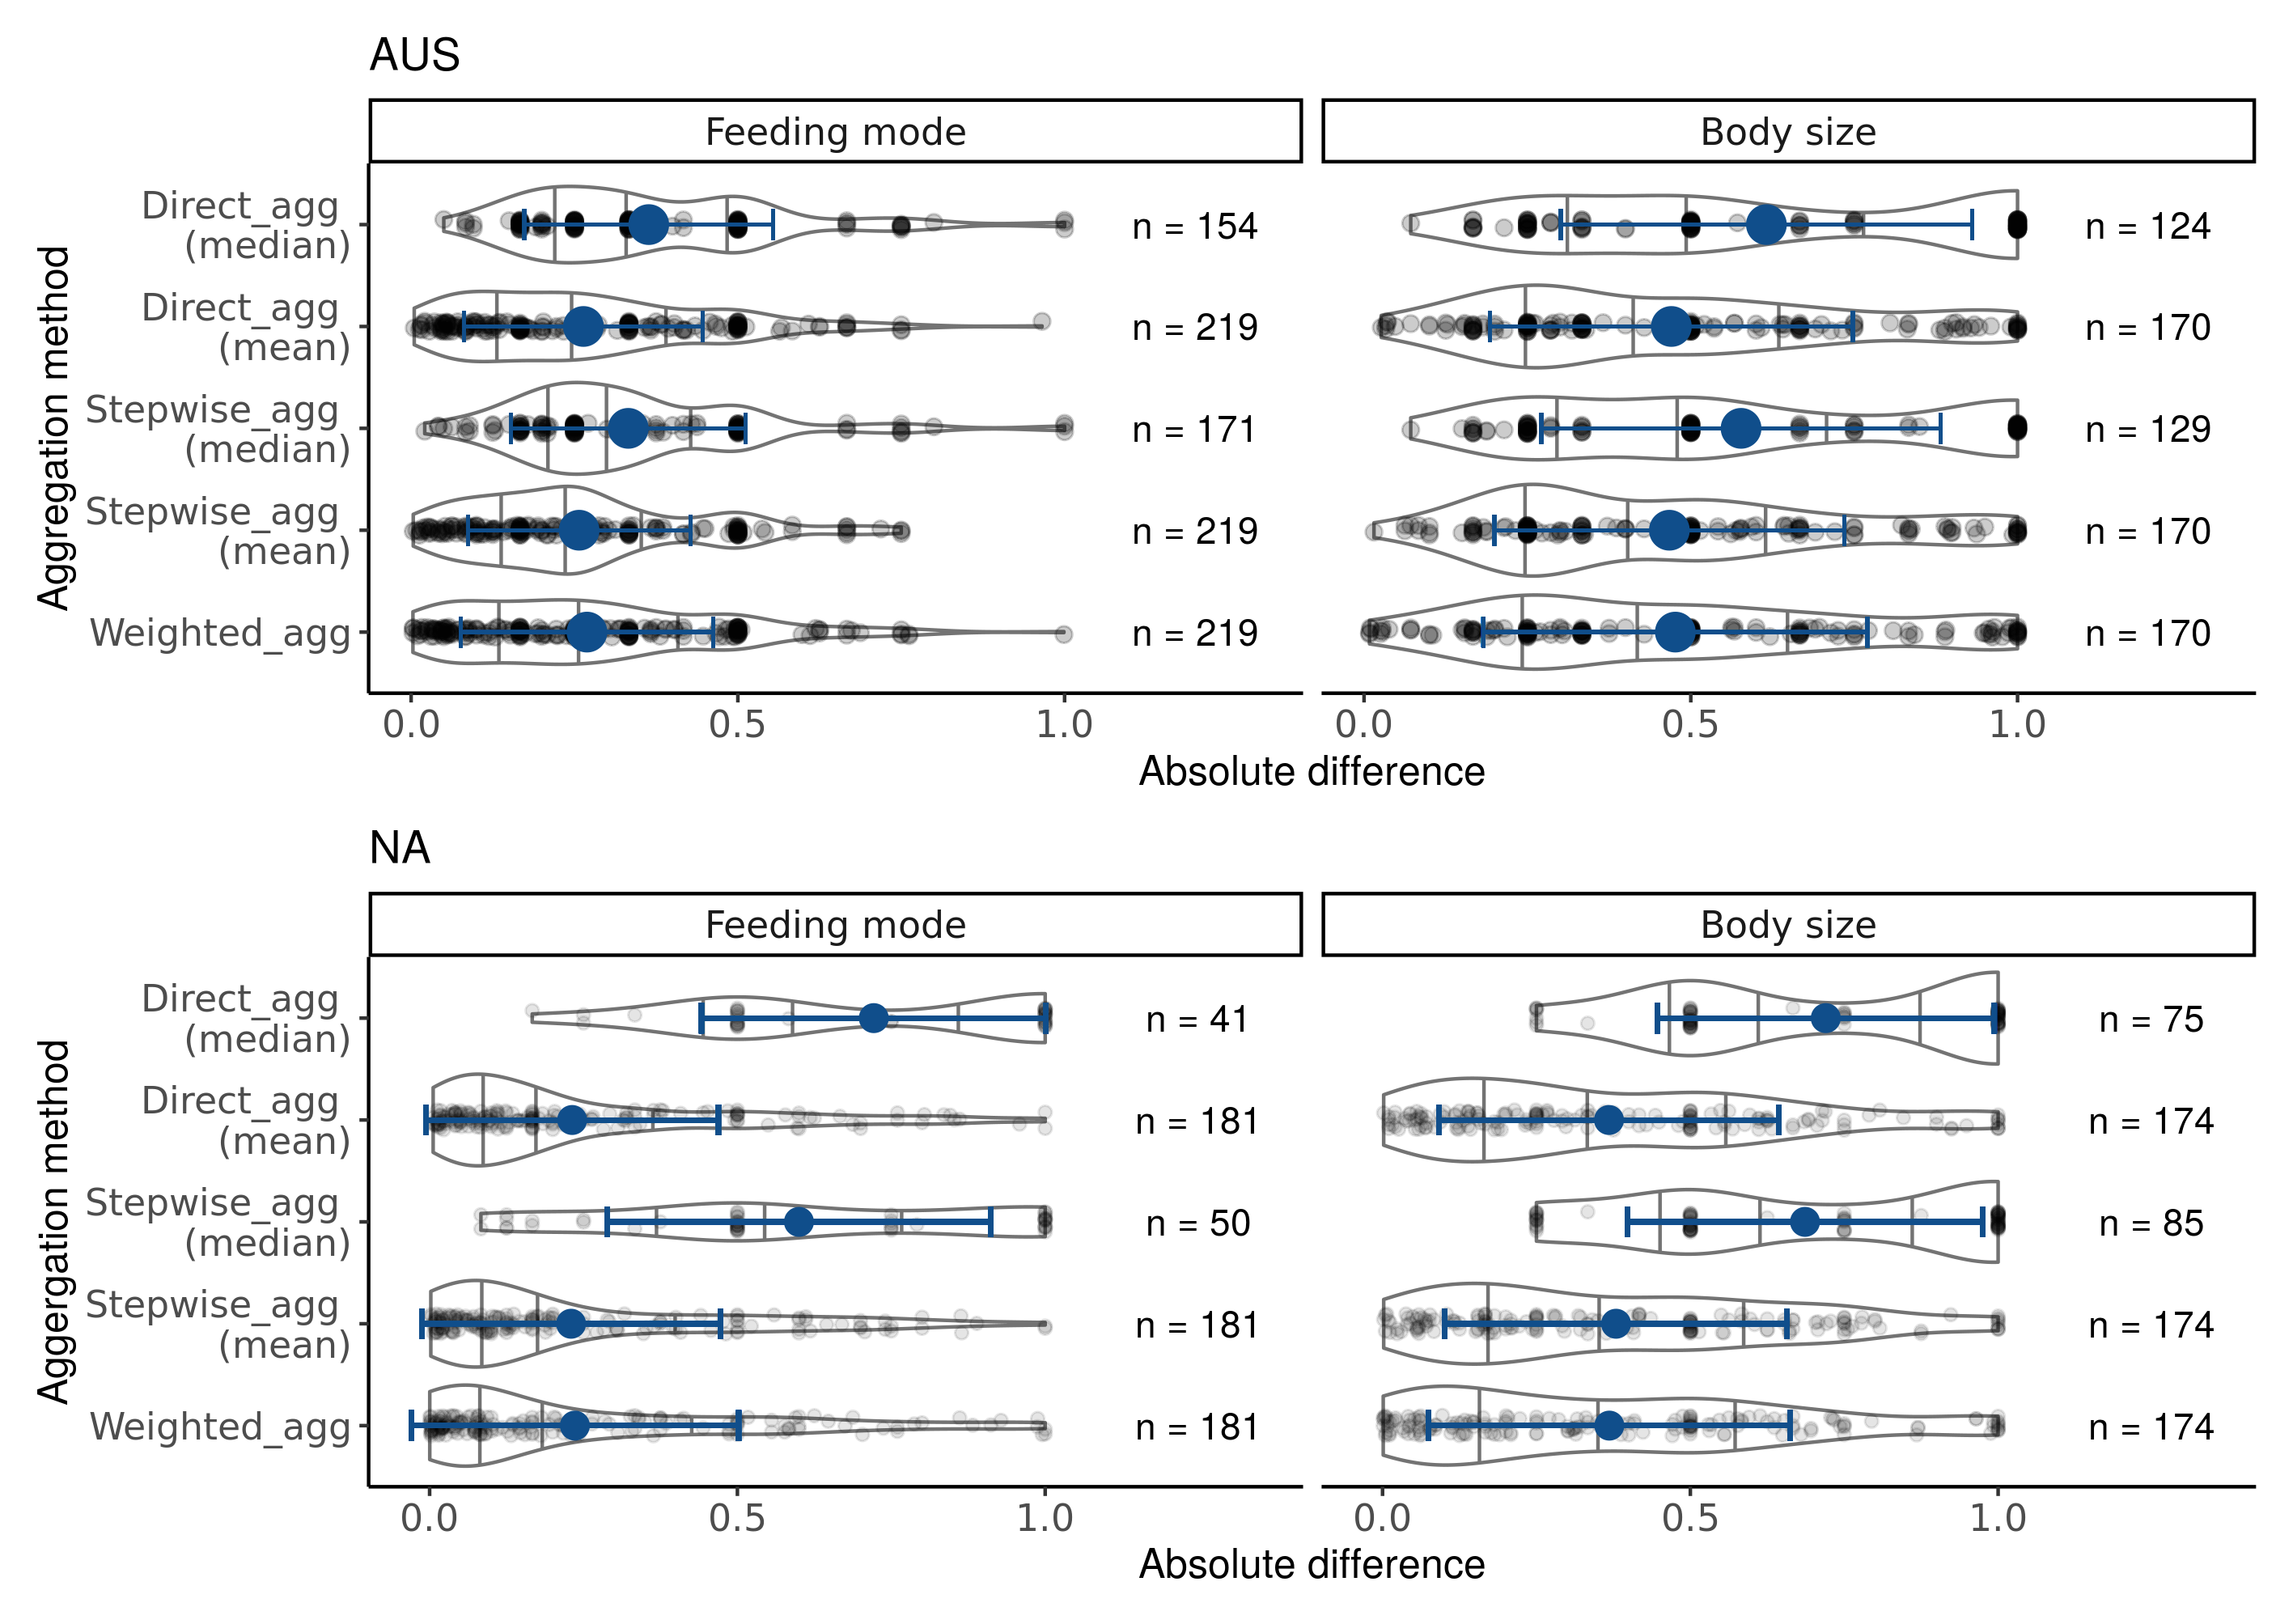
\includegraphics[width=16.5cm, height=12cm]{Deviances_trait_agg_combined.png}
  \caption{Cases (factor combination of investigated families and traits) where differences occurred between aggregated traits and expert assigned traits at family level for the Australian and North American dataset. Violin plots - mirrored density plots - show the density of the absolute trait affinity differences for the grouping features feeding mode and body size. Results for the North American dataset for the grouping features locomotion, respiration, and voltinism are shown in the supporting information (Figure \ref{fig:diff_aggr_traits_pyne}). Absolute differences in trait affinities are depicted as grey dots. \textit{n} denotes the number of cases per comparison where differences occurred. The blue dot indicates the mean of absolute differences, and the error bars show the standard deviation. The grey vertical lines show the 25\textsuperscript{th}, 50\textsuperscript{th} and 75\textsuperscript{th} quantiles of the density estimate. Abbreviations: AUS, Australia; NA, North America.}
  \label{fig:diff_aggr_traits_combined}
\end{figure}

\newpage

%%%%%%%%%%%%%%%%%%%%%%%%%%%%%%%%%%%%%%%%%%%%%%%%%%%%%%%%%%%%%%%%%%%%%%%%%%%%%%%%%%%%%%%%%%%%%%%%%%%%

\subsection*{Effects of harmonisation and trait aggregation on inferences regarding trait-environment relationships}

Our re-analysis of the \citet{szocs_effects_2014} study on the effects of salinisation on invertebrate traits showed that the use of harmonised and aggregated trait data may be useful for ecological studies on trait–environment relationships. Overall, harmonised trait data and all aggregation methods produced similar distributions of RDA species scores (\ref{fig:violin_plot_species_sc}) compared with the original analysis, and they resulted in similar, but fewer, traits that distinguished upstream and downstream sites than the original analysis (Figures \ref{fig:violin_plot_species_sc} and \ref{fig:boxplot_scores_on_constrained_axis}).

RDA using harmonised, but not aggregated, grouping features identified some, but not all, of the same traits that were identified by the original analysis (Figures \ref{fig:violin_plot_species_sc} and \ref{fig:boxplot_scores_on_constrained_axis}). The original RDA in \citet{szocs_effects_2014} indicated that downstream sites (higher salinity) were characterised by the traits: ovoviviparity, multivoltinism, long life-cycle duration ($> 1$ year), shredder, and gill respiration, whereas RDA with the harmonised data identified the first three traits but did not include shredder or gill respiration traits. The original RDA indicated that upstream sites (lower salinity) were characterised by the traits: univoltinism, oviposition in clutches, and short life-cycle duration ($< 1$ year), and RDA with the harmonised data characterised upstream sites by univoltine taxa with short life-cycle durations that lay their eggs in an aquatic environment (aquatic eggs). This difference in the oviposition trait is not substantial because the trait aquatic eggs of the harmonised grouping feature oviposition was derived by combining the trait oviposition in clutches and other related traits (Table \ref{tab:traits_harmonisation}).

RDA based on harmonised traits that were aggregated to family level also produced results similar to the original analysis but with fewer traits distinguishing upstream and downstream sites (Figures \ref{fig:violin_plot_species_sc} and \ref{fig:boxplot_scores_on_constrained_axis}). The \textit{direct\_agg\textsubscript{mean}}, \textit{direct\_agg\textsubscript{median}}, and \textit{weighted\_agg} characterised the downstream sites with the same traits as the original analysis except the trait shredder. As for the RDA with harmonised but not aggregated data, RDA with these three aggregation methods characterised upstream sites by the traits univoltinism, short life-cycle duration, and aquatic eggs. The \textit{stepwise\_agg\textsubscript{mean}} and \textit{stepwise\_agg\textsubscript{median}} methods produced the same results except that none of the life-cycle traits characterised upstream or downstream sites. Thus, compared with the original study’s findings, aggregating by the direct and weighted methods yielded less change than the stepwise methods in interpretation of the RDA results.

\begin{figure}[H]
    \centering
    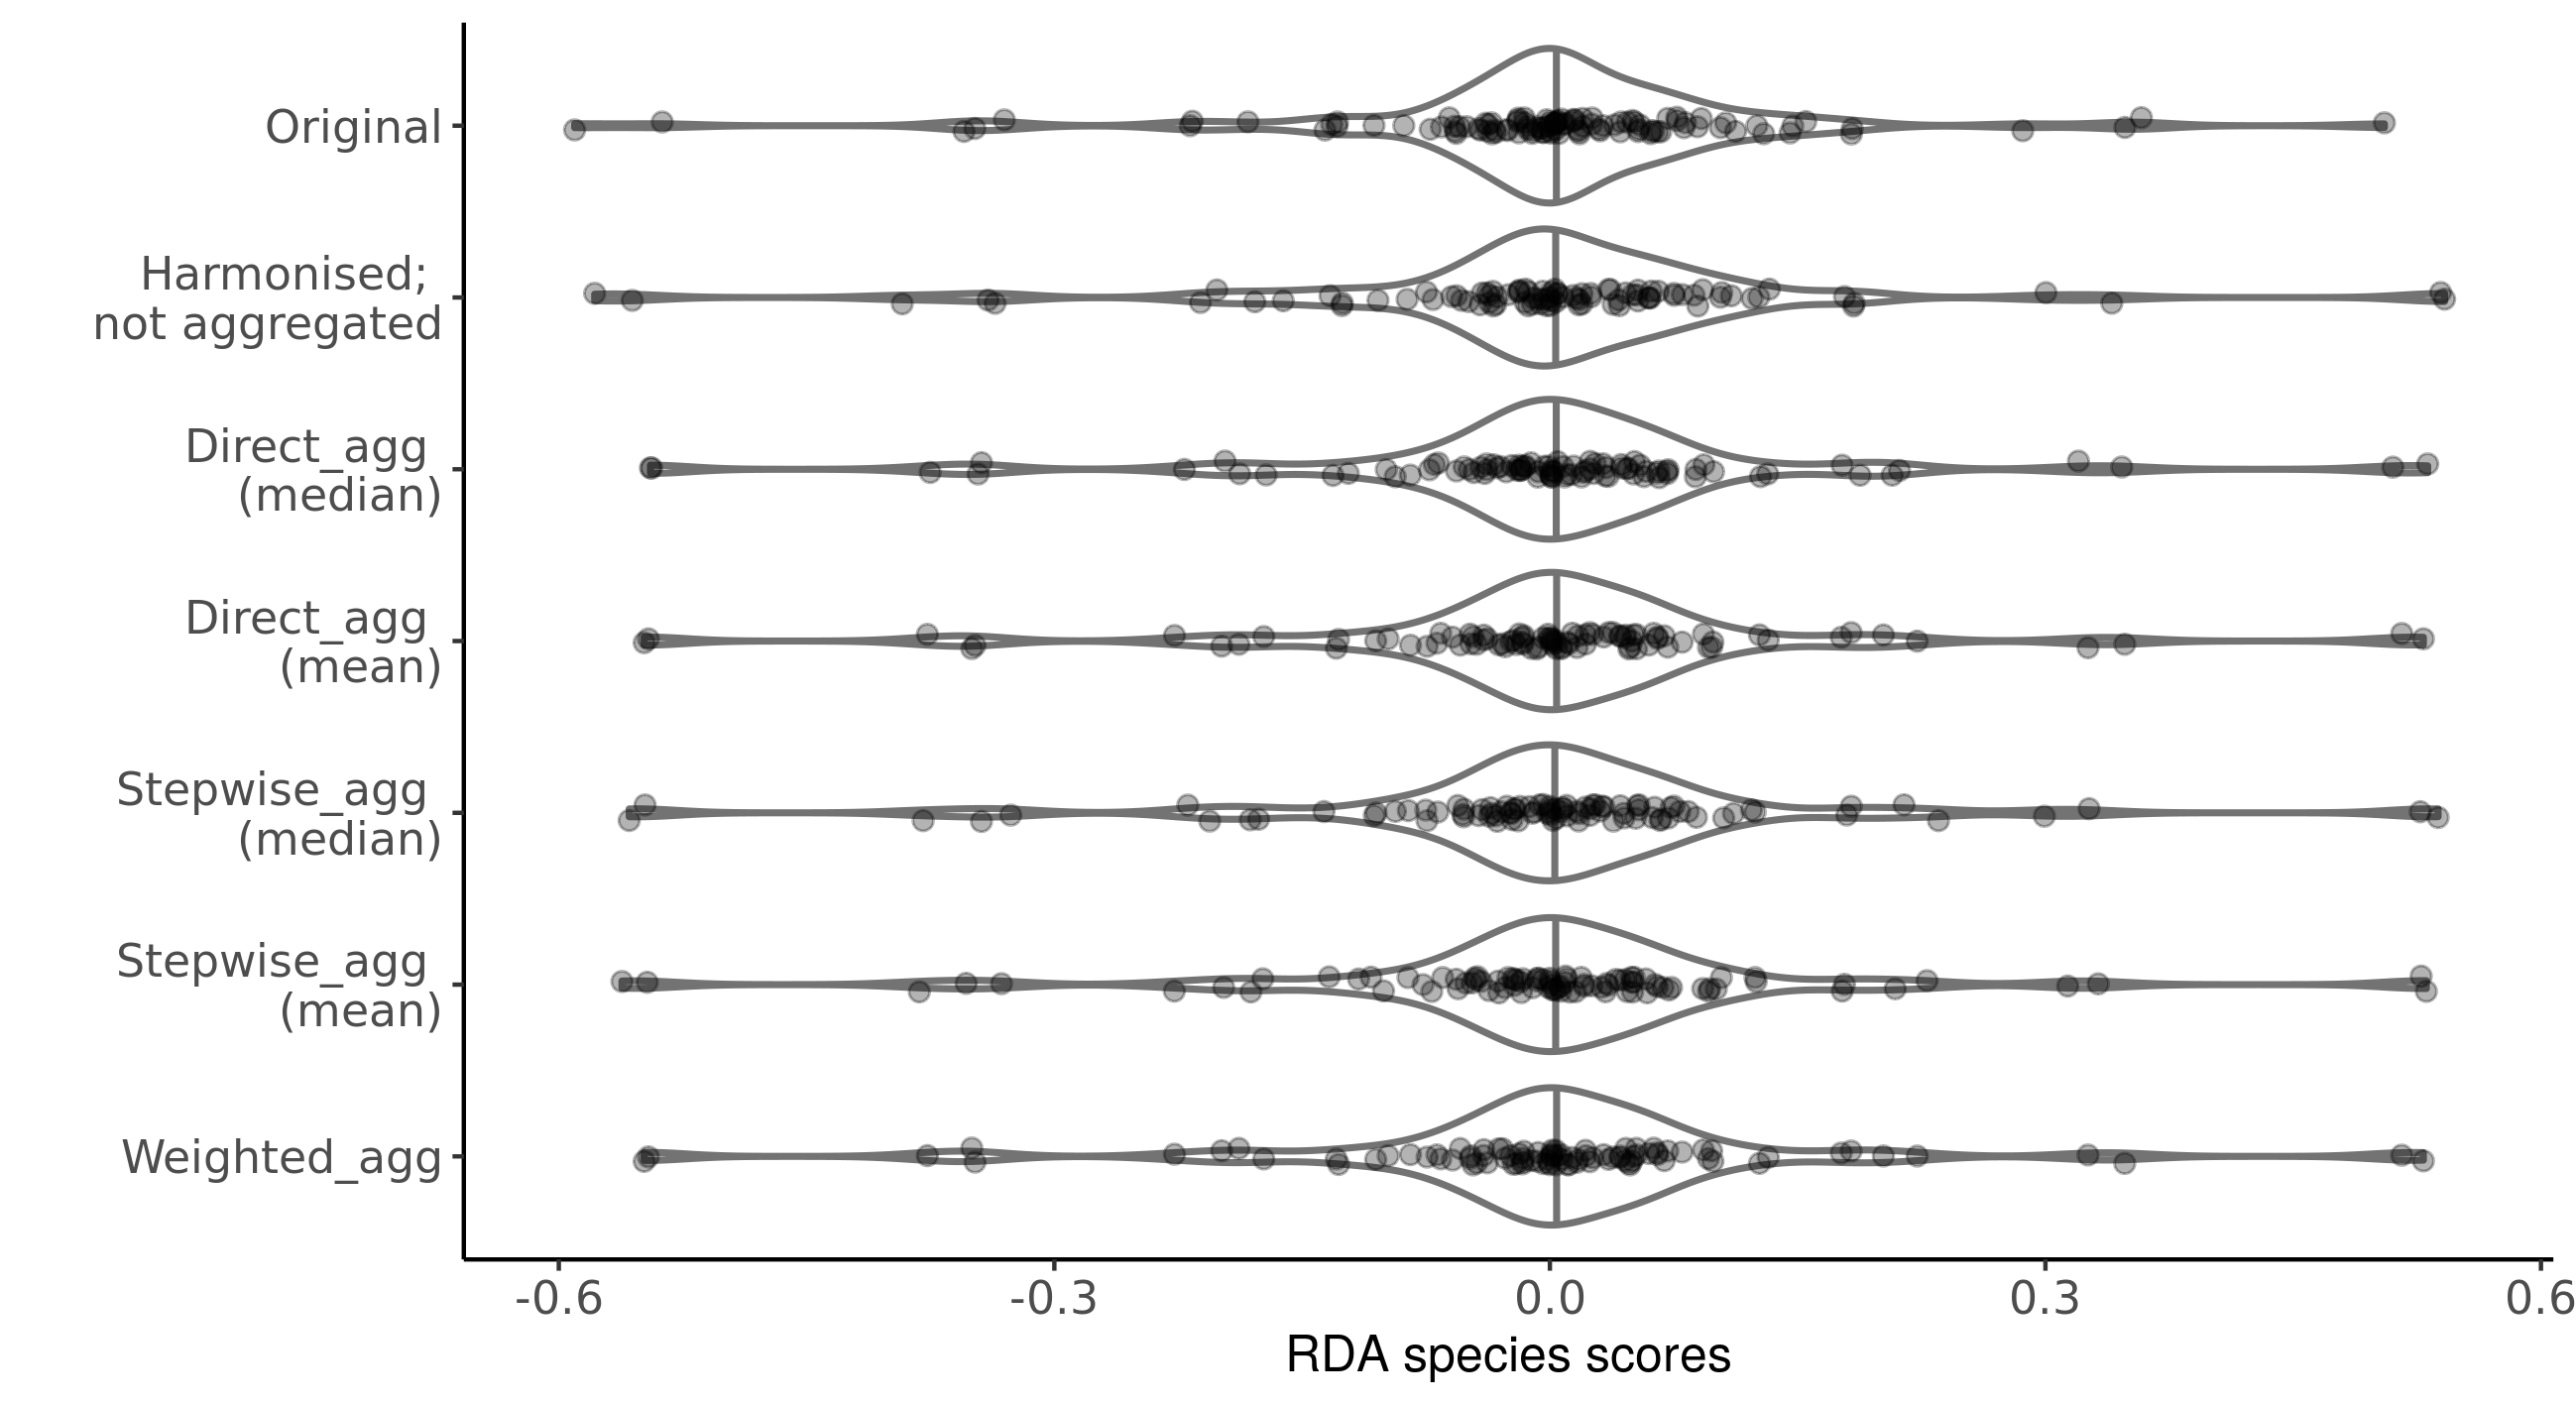
\includegraphics[width=16.5cm, height=10cm]{Species_scores_rda.png}
    \caption{Species scores obtained by RDA from the original analysis (\cite{szocs_effects_2014}), using harmonised grouping features, and using harmonised grouping features with traits aggregated to family level with five different aggregation methods. The dots represent the individual species scores for each analysed trait along the conductivity axis. The violin plot shows the density estimate of the species scores. Grey vertical lines indicate the median of the obtained species scores.}
    \label{fig:violin_plot_species_sc}
\end{figure}

\begin{figure}[H]
  \centering
  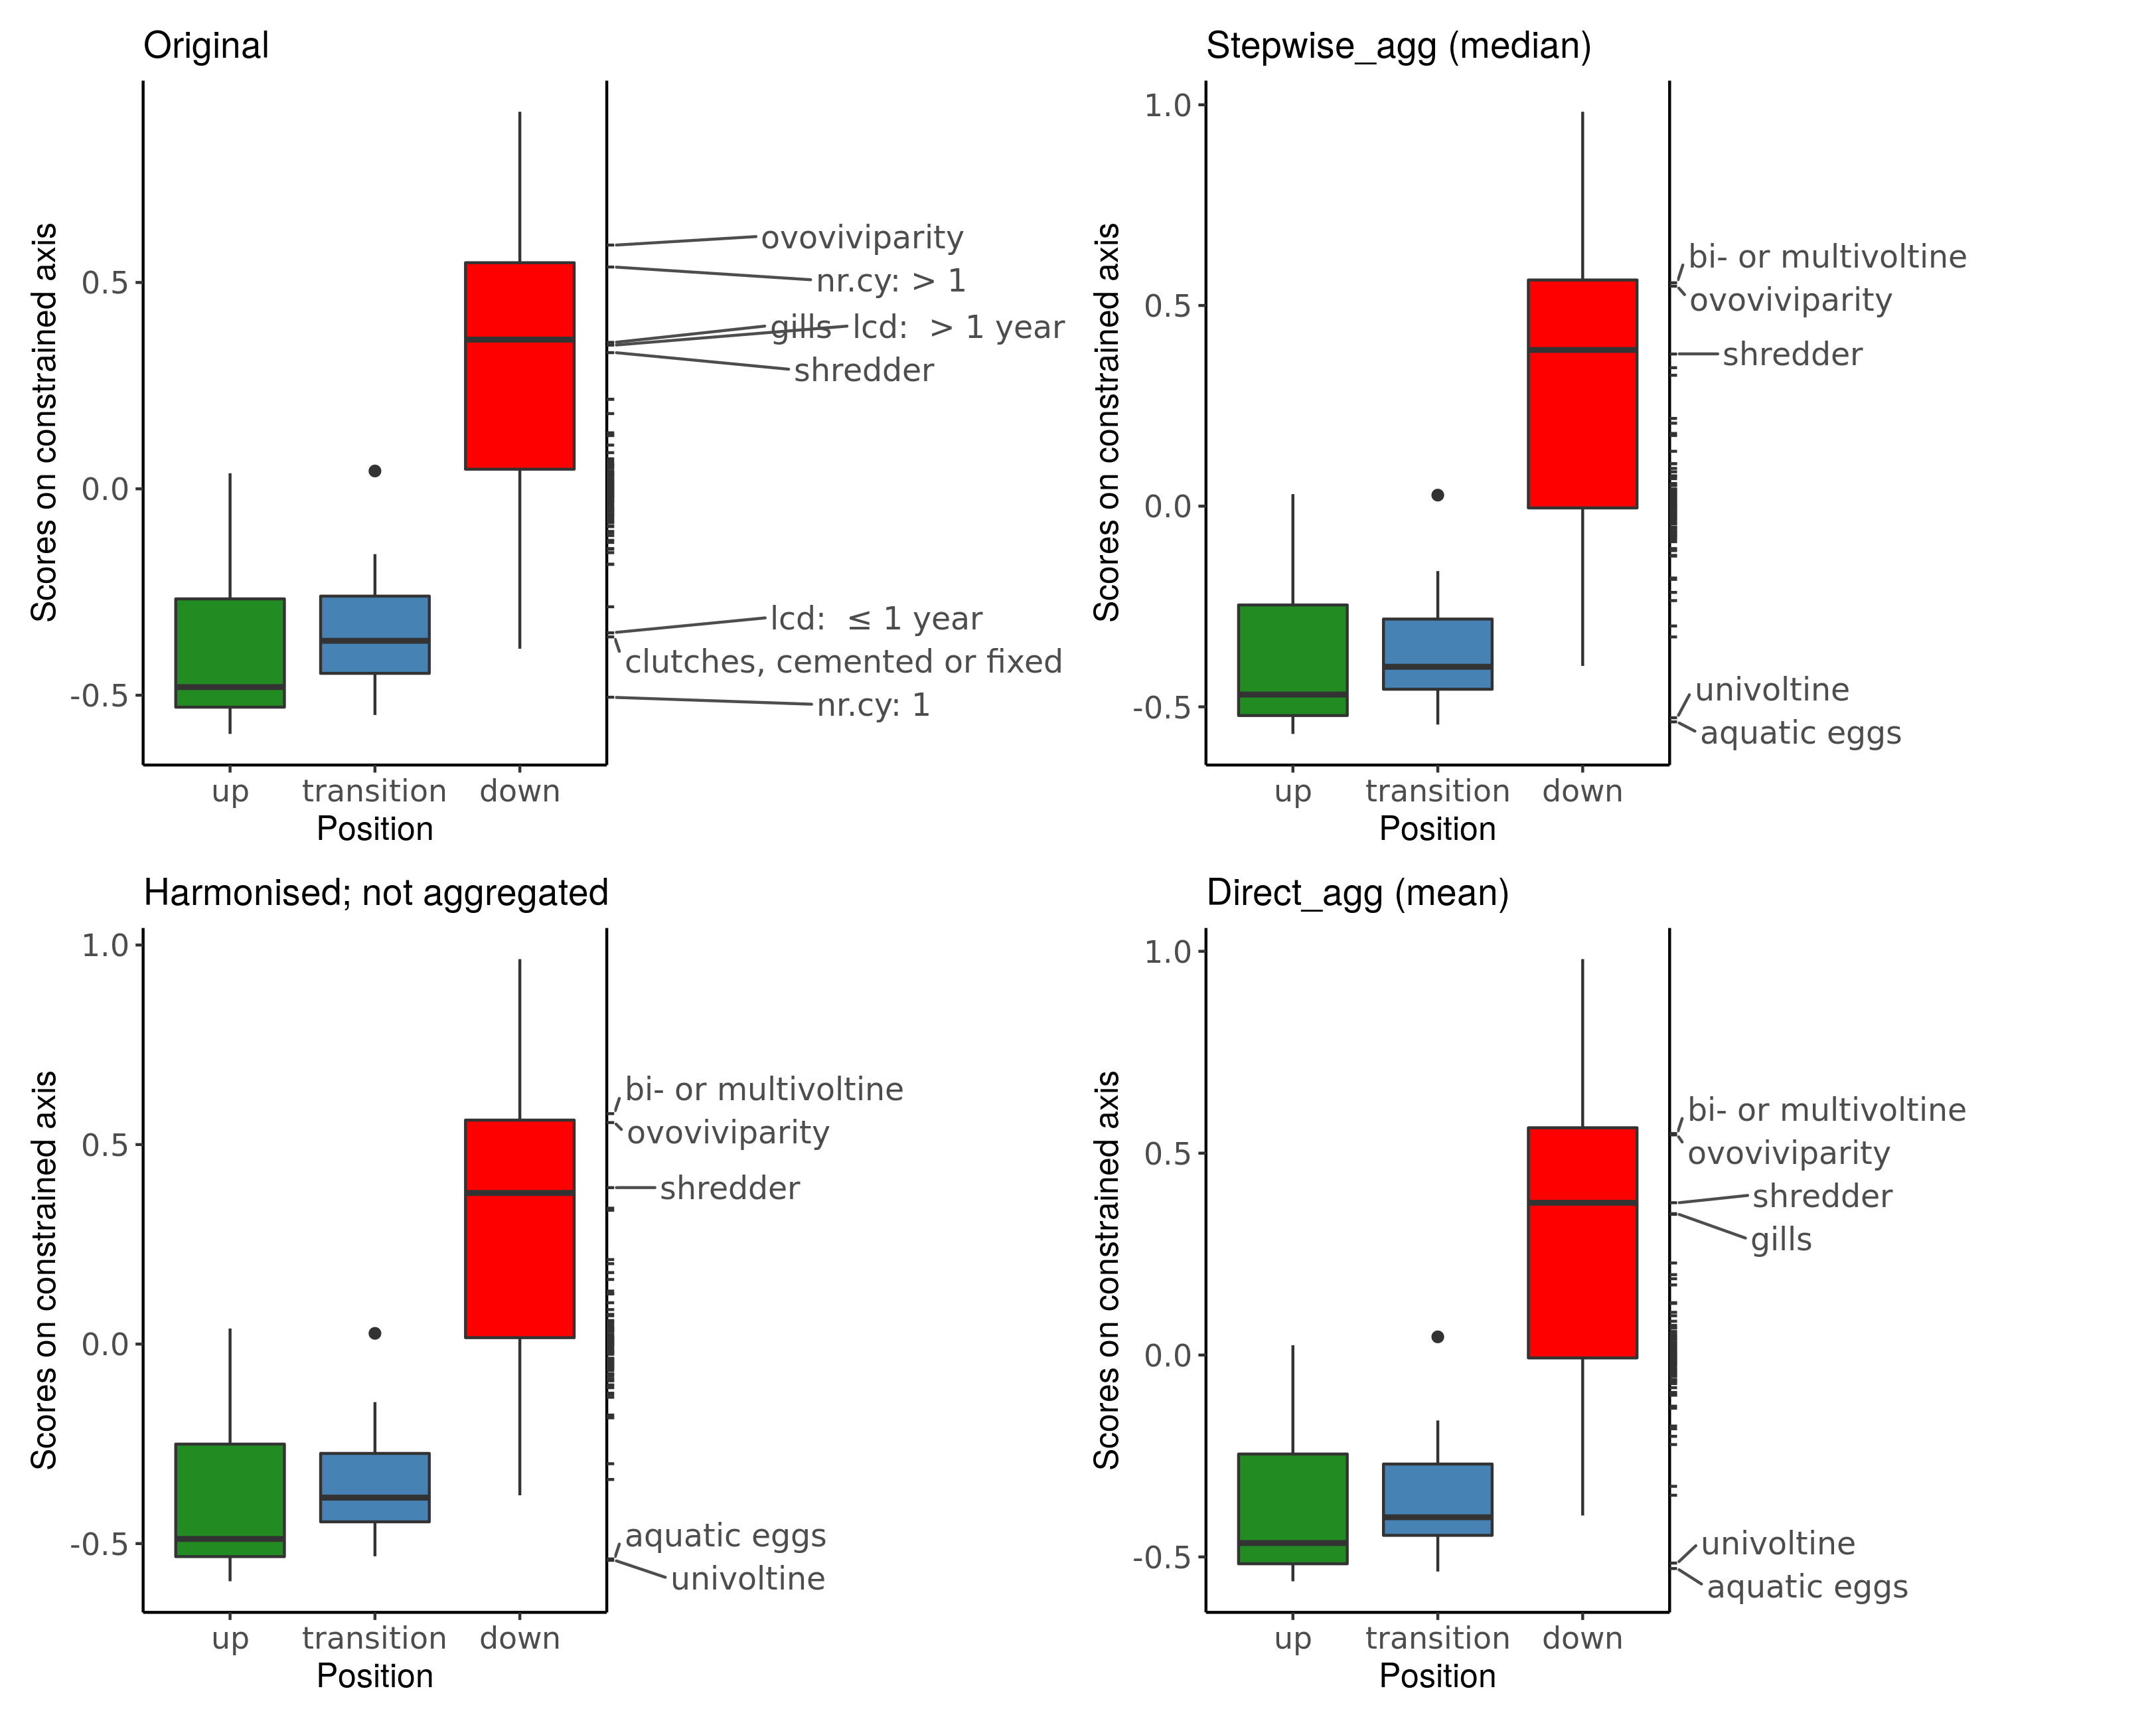
\includegraphics[width=17cm, height=14.5cm]{boxplot_scores_combined.png}
\end{figure}
\begin{center}
\captionof{figure}{RDA of traits constrained by electric conductivity for harmonised but not aggregated data, data aggregated with \textit{stepwise\_agg \textsubscript{median}} (largest difference in terms of responsive traits to salinity to the original study), data aggregated with \textit{direct\_agg \textsubscript{median}} (smallest difference in terms of responsive traits to salinity to the original study), and the original study. Shown are boxplots of the site scores along the conductivity axis. The rug on the right side of each plot indicates species scores of the traits on the conductivity axis. Only traits with a Mahalanobis distance greater than the $97.5 \%$ quantile of the Chi-square distribution (5.02) were labelled. For better comparability, species scores of the original analysis were multiplied by -1. Results for the other aggregated methods are shown in the supporting information (Figure \ref{fig:boxplots_scores_on_constrained_axis_REMAIN}). Abbreviations: lcd, life cycle duration; nr.cy, potential number of cycles per year.}
\label{fig:boxplot_scores_on_constrained_axis}
\end{center}

Calculating FD metrics for the original, harmonised (not aggregated), and aggregated datasets showed that the use of harmonised trait data results in similar FRic and FDiv values compared to the original dataset ($R2 = 0.96$ and $0.86$, respectively). Generally, aggregated trait data yielded lower, but moderate to good, correlations to the original for FRic and FDiv than the harmonised (Figure \ref{fig:FRic} and \ref{fig:FDiv}). 
By contrast, FEve calculated with harmonised and aggregated trait data seemed to substantially differ from the original dataset (all correlations below $< 0.1$), except for \textit{stepwise\_agg \textsubscript{median}}, which had an $R2$ of 0.48 (Figure \ref{fig:FEve}).  


% Evaluated by R2


\newpage

%%%%%%%%%%%%%%%%%%%%%%%%%%%%%%%%%%%%%%%%%%%%%%%%%%%%%%%%%%%%%%%%%%%%%%%%%%%%%%%%%%%%%%%%%%%%%%%%%%%%

\section*{Discussion}

Freshwater invertebrate trait databases are a valuable source of data that are freely available to researchers and that can offer opportunities for large-scale, cross-regional ecological study without the need for time-consuming and expensive field work. However, a lack of consistency among regional and continent-wide databases in trait definitions, trait affinity coding, and taxonomic resolution can greatly limit the use of combined databases. We explored the effects of harmonising grouping features and aggregating trait affinities at different taxonomic levels from databases from four different continents on the outcomes of trait affinities and on analysis of trait–environment relationships. We found that despite discrepancies in trait definitions and taxonomic resolution across databases, harmonised and aggregated data were generally effective in identifying trait–environmental relationships, as evidenced by similar results from RDA as were found using observational data. Our results have implications for future multi-regional ecological studies that may benefit from the use of existing databases and provide insight into methods for harmonising traits with differing trait definitions and selecting aggregation methods that minimize either cases or ranges of differences in trait affinity scores when aggregating from higher to lower taxonomic precision.

\subsection*{Harmonising trait databases}

Synthesising trait information from multiple trait databases is crucial for developing the full potential of trait-based approaches, such as for studying community trait responses to environmental gradients across geographic regions. Others have noted the lack of standardised trait terminology in freshwater ecology (\cite{baird_toward_2011, brink_traits-based_2011}), but in this study we show for the first time the discrepancies that exist across some commonly used grouping features. Furthermore, we offer insight into the need for, and process of, harmonising invertebrate trait information from trait databases of different regions. Some of the challenges we found were that grouping features were resolved differently into traits in different databases and that various codings (fuzzy, categorical, binary) were used to describe traits. In addition, the same traits were sometimes defined differently, requiring expert knowledge to reclassify these traits (e.g. the trait piercer). Missing information was another challenge. We aimed to use most of the available invertebrate trait information for different regions to establish harmonised grouping feature datasets, but the availability of trait information varied strongly across grouping features and databases. For instance, extensive information was available for grouping features that are often used in trait–environment studies, such as feeding mode and respiration, but there was surprisingly little information on body form, a trait that is relatively easy to characterise.

To resolve definition discrepancies and facilitate data synthesis in the future, terminological standards are needed. Harmonised definitions and concepts of traits have been developed in the past for other organism groups, such as for plants with the \textit{Thesaurus of Plant Characteristics} (TOP) initiative (\cite{garnier_towards_2017}). The core of this harmonisation initiative is to provide standardised trait definitions and to draw connections to synonyms, related terms, and surrounding concepts by linking to other controlled vocabularies or ontologies in the field. Such initiatives should encourage freshwater ecologists to establish unambiguous terminologies for invertebrate traits. The existing freshwater invertebrate trait databases could be linked through standardised terminologies or ontologies, as suggested by \citet{baird_toward_2011}. By following the recently proposed \textit{Ecological Trait-data Standard Vocabulary} (ETS), providers of invertebrate trait data could connect their traits to such ontologies (\cite{schneider_towards_2019}). Once standardised trait definitions are established, they will improve trait data sharing, trait data processing when working with multiple trait databases, and, ultimately, interpretation of the derived results. 

% %%%%%%%%%%%%%%%%%%%%%%%%%%%%%%%%%%%%%%%%%%%%%%%%%%%%%%%%%%%%%%%%%%%%%%%%%%%%%%%%%%%%%%%%%%%%%%%%%%%%%%

\subsection*{Trait aggregation method choice}

The taxonomic resolution used to describe the occurrence and abundance of freshwater invertebrates can be highly variable because species-level identifications require specialists and are also often time-consuming and expensive (\cite{marshall_taxonomic_2006, resh_which_2008}). Consequently, trait information at the family level has been widely used by freshwater ecologists, for example in bioassessment (\cite{beketov_spear_2009}).
However, traits assigned at the family level may not reflect the full trait diversity that exists within, for example, large, ecologically diverse families such as Chironomidae (\cite{serra_synthesising_2016}). Additionally, various trait aggregation methods have been used by researchers to compare trait profiles based on different taxonomic levels. Evaluation of the differences between aggregated and assigned traits is difficult because it remains unclear what the true value of a particular trait is for a particular family. Aggregation of trait information at the species or genus level to a single estimate at the family level implies a precision that is not necessarily present, especially not for traits with high variability or if trait information at species level is missing. Indeed, some traits can vary strongly at more resolved taxonomic levels than the family level. For example, \citet{monaghan_improving_2013} found high intra-family trait dispersion in the Tachet database for traits within the grouping features body size, flow preference, and reproduction. Furthermore, studies focusing on the lability of traits, (i.e. how much traits are constrained by phylogeny), found that traits of ecological preferences (e.g. thermal preference), body size, resistance forms, and, to a lesser extent, feeding mode are labile, and thus possibly highly variable (\cite{poff_functional_2006, wilkes_traitbased_2020}). 

If trait aggregation is necessary, however, our study offers insights about the circumstances under which the choice of aggregation method may be important. The 5 aggregation methods we tested used either the mean or the median and different weightings to assign family-level affinities. Our results indicated that for both the Australian and North American datasets (1) the median aggregation methods provided affinities that were often closer to the assigned traits than were those provided by the mean aggregation methods and (2) the different weighting approaches exerted only a minor influence on the aggregated trait affinities. However, when differences occurred between median aggregation methods and assigned traits, these differences were greater in absolute value compared with the mean aggregation methods, particularly for the North American dataset where mean absolute differences for median aggregations were twice as high as for mean aggregations. This pattern of greater differences for median than mean aggregations is probably caused by the use of binary coding in the North American trait dataset and by the assigned traits. Binary coded traits have affinities of either 1 or 0; therefore, traits of a particular grouping feature showed, in most cases, a higher difference in trait affinities to each other than if they were fuzzy coded. Median-aggregated binary-coded taxa often resulted in a value of 0 or 1, whereas mean aggregation often yielded values between 0 and 1. Thus, using the median resulted in the North American dataset either to agreement with the assigned traits or to more substantial differences compared to the use of mean aggregation methods. This pattern inherent in using median-aggregation methods to aggregate binary-coded data should be considered when researchers choose methods to resolve affinities at different taxonomic levels. 

We expected that, in addition to averaging measures, different weighting approaches to aggregation (i.e., equal weight to each taxon, equal weight to each genus, or weighted by number of species) would affect affinities for families with varying phylogenetic structure. However, we found through simulations that trait variability had a greater effect on the range of affinities (i.e., greater ranges of affinities at higher levels of variance) and on the differences in affinities between weighting approaches. In the simulation, taxonomic structural unevenness appeared to produce some variation in affinities among weighting approaches, especially for a family where one genus had a much larger number of species than its other genera. The comparison between aggregated and assigned traits showed, that the number of differing cases and the mean absolute differences in trait affinities, as well as the distributions of absolute trait affinity differences to assigned traits, were similar across the mean aggregation and across the median aggregation methods, which suggests a small influence of the weighting approach on the aggregation outcomes. The minor impact of the weighting approaches on trait aggregation might be explained by the fact that a considerable portion of taxa had low numbers of genera or species. Of the taxa that were compared from the North American trait dataset, 14 \% were identified at family and 62 \% at genus level, 52 \% comprised five or fewer genera, and 13 \% contained just one genus (Figure \ref{fig:tax_hierarchy_NOA}). In the Australian dataset, 21 \% of the compared taxa were identified at family, 40 \% at genus, and 39 \% at species level, 68 \% of the taxa contained five or fewer genera, and 40 \% just one genus (Figure \ref{fig:tax_hierarchy_AUS}). Hence, these results could change when more species-level trait information becomes available. Our findings show that the choice of aggregation method may matter less when phylogenetic structure is fairly even and traits are less variable, but the \textit{stepwise\_agg\textsubscript{median}} method tended to produce the widest range in affinities, especially with high taxonomic unevenness and high trait variability. 

\subsection*{Using harmonised and aggregated datasets for ecological research}

By reanalysing trait–environment relationships identified in \citet{szocs_effects_2014} with our harmonised and family-level aggregated datasets, we illustrated the potential for the use of harmonised and aggregated data in ecological research. As far as we are aware, ours is the first study to compare inferences regarding trait–environment relationships based on harmonised and non-harmonised data. Our re-analysis of the data on salinisation effects on biological traits yielded only slightly different results compared with the original study, which agrees with previous findings that family-level traits can be sensitive enough to detect environmental impacts (\cite{beketov_spear_2009}). However, some of the traits that had responded in the original analysis did not respond in the re-analysis, specifically feeding mode shredder, respiration gills, and life-cycle duration traits. There are several possible reasons for these discrepancies. The non-responsive traits were those closest to the threshold for association with either higher or lower salinity, and so the precision lost through trait harmonisation may have decreased our ability to detect a relatively weak association. The shredder feeding mode was the only trait that was non-responsive when using harmonised (but not aggregated) data as well as when using aggregated data. This result was likely because of the harmonisation procedure, in which this trait was combined based on three traits (miner, xylophagus, and shredder) used in the original databases. Consequently, the trait affinities in the original data had a higher mean and standard deviation than in the harmonised and aggregated data (Table \ref{tab:SI_resp_traits_summary_stats}), suggesting that the signal in the original data was weakened by harmonisation. Given this result, we suggest that if harmonisation is necessary, harmonised and non-harmonised data, if available, should be compared, and possible averaging effects should be considered in further analyses. However, our results also illustrate that where site-level data are not available, harmonised and aggregated datasets may be useful in identifying at least the strongest associations between traits and environmental conditions. 

%%%%%%%%%%%%%%%%%%%%%%%%%%%%%%%%%%%%%%%%%%%%%%%%%%%%%%%%%%%%%%%%%%%%%%%%%%%%%%%%%%%%%%%%%%%%%%%%%%%%%%%

\subsection*{Outlook}

Although comprehensive freshwater invertebrate trait databases have been developed for several regions in the past, data synthesis presents challenges because of discrepancies in trait definitions, coding of trait affinities, and taxonomic resolution. By providing an overview of definition discrepancies, we have set a starting point for the development of standardised trait terminology through which invertebrate trait databases can be linked. Agreement on standard terminology and the subsequent development of ontologies are the next steps to facilitate trait-based analysis at large geographical scales. As our analysis showed, some grouping features might need to be re-classified to fit into such a standardised terminology. Although we showed that trait affinities from fuzzy and binary coding can be used together, we also recommend that a uniform coding of traits should be addressed during trait standardisation. 

As ecological knowledge increases, and with the help of new methods such as computer vision for species and trait identification (\cite{hoye_deep_2020}), more observed taxa will be identified to the species level and trait data will be available at the species level in the future, reducing the need for trait aggregation. However, we showed that trait aggregation is often in agreement with expert assignments, especially through aggregation approaches that use the median. Based on this analysis, we cannot claim that a specific aggregation method is objectively the best, and except for cases where traits are highly variable and phylogenetic structure is highly uneven, the choice of aggregation method does not appear to be influential to the outcome. Weighting trait information based on the taxa present in the database used does not seem to have much influence except when the phylogenetic structure is highly uneven. However, we recommend that the type of coding used to describe traits (binary, fuzzy) should be considered, because median and mean aggregations can yield very different results for binary-coded traits. We also suggest that a measure of trait dispersion should be reported to indicate the uncertainty of the aggregated estimate. Use of carefully harmonised and integrated trait data as described here should enhance our ability to study a wide range of large-scale ecological questions with greater rigor than currently exists.
 
%%%%%%%%%%%%%%%%%%%%%%%%%%%%%%%%%%%%%%%%%%%%%%%%%%%%%%%%%%%%%%%%%%%%%%%%%%%%%%%%%%%%%

\section*{Acknowledgements}

We thank Brooke Cassell for technical editing of the manuscript. The project, in which this study was conducted, is funded by the German research society (DFG, project number 338785727).

\section*{Data availability statement}

Harmonised invertebrate trait datasets for Australia, Europe, North America and New Zealand are deposited in the Github repository: \url{https://github.com/KunzstLD/Trait-aggregation}.

\section*{Conflict of interest}

The authors declare no conflict of interest.

\section*{Author contribution}
R.B.S. and S.K. designed the study; B.J.K. and L.M. provided trait data for Australia; P.U-P. provided body form trait data for European and North American invertebrates; C.P.H., N.L.P., and L.T. provided trait data for North America; C.D.M. provided trait data for New Zealand;
B.J.K., A.S-K., C.D.M, W.G., N.L.P., L.M., and C.P.H. provided in depth information on trait data and discussed the procedure of analysis; S.K. conducted data processing and the statistical analyses.; S.K. wrote the manuscript; B.J.K, A-S.K., C.D.M, P.U-P., C.P.H., and R.B.S. discussed the results and provided suggestions on the manuscript.

\newpage

%%%%%%%%%%%%%%%%%%%%%%%%%%%%%%%%%%% Bibliography %%%%%%%%%%%%%%%%%%%%%%%%%%%%%%%%%%
\printbibliography

\newpage

%%%%%%%%%%%%%%%%%%%% Tables %%%%%%%%%%%%%%%%%%%%%%%

\section*{Tables}

% Table 1
\begin{landscape}
  \begin{longtable}{m{2.0cm}|m{4.0cm}|m{4.2cm}|m{4.2cm}|m{1.7cm}|m{2cm}|m{2.2cm}}
      \caption{Excerpt of the comparison of trait definitions between invertebrate trait databases for the traits predator and swimming. The definition is quoted if it enables differences to be identified, otherwise the differences are described. The full version and further information can be found in the supporting information Table \ref{stab:trait_definitions}.}
      \label{tab:trait_definitions}
      \endfirsthead
      \toprule[.1em]
      Trait & \specialcell{Freshwater- \\ ecology.info} & Tachet & CONUS & Vieira & Australia & \specialcell{New \\ Zealand} \\
      \toprule[.1em]
      Feeding predator & 
        "Eating from prey" & 
        \begin{itemize}
            \item Carvers, engulfers \& swallowers
            \item Piercers (plants \& animals) are an additional trait
        \end{itemize} & % Notes: Tachet -> Piercer (plants & animals)
        Engulfers ("ingest prey whole or in parts") \& 
        piercers ("prey tissues and suck fluids") & 
        Predator &
        Piercer \& engulfer &
        Predator
        \\ 
        \midrule
        Locomotion swimming & 
        \begin{itemize}
            \item Passive movement like floating or drifting (trait swimming/scating)
            \item Active movement (trait swimming/diving)
        \end{itemize}. &
        \begin{itemize}
            \item Surface swimmers (over and under the water surface)
            \item Full water swimmers (e.g. Baetidae).
        \end{itemize} & 
        "Adapted for "fishlike" swimming" & 
        Swimmer & 
        Traits swimmer and skater & 
        Swimmers (water column)
        \\
      \bottomrule
  \end{longtable}
\end{landscape}

% Table 2
\begin{longtable}{m{2.5cm}|m{4cm}|m{7.5cm}}
\caption{Traits of harmonised grouping features from six invertebrate trait databases and four geographic regions. The last column indicates traits that were combined for harmonisation (no combining needed if empty).}
\endfirsthead
\toprule[.1em]
\label{tab:traits_harmonisation}
%\begin{tabular}
\specialcell{Grouping \\ feature} & Trait & Combined traits\\
\toprule[.1em]
Voltinism    & \begin{tabular}[c]{@{}l@{}}Semivoltine\\ Univoltine\\ Bi/multivoltine\end{tabular}                                & \begin{tabular}[c]{@{}l@{}}\textless 1 generation per year\\ 1 generation per year\\ \textgreater 1 generation per year\end{tabular}                                                                                                                                            \\
\midrule
Body Form    & \begin{tabular}[c]{@{}l@{}}Cylindrical \\ Flattenend\\ Spherical\\ Streamlined\end{tabular}                       & \begin{tabular}[c]{@{}l@{}}Cylindrical, tubular\\ Flattenend, dorsoventrally flattened$^{\dagger}$ \\ Spherical, round (humped)\\ Streamlined, fusiform\end{tabular}                                                                                                                                                                          \\
\midrule
Size         & \begin{tabular}[c]{@{}l@{}}Small \\ Medium \\ Large\end{tabular}                                                  & \begin{tabular}[c]{@{}l@{}}\textless 9 mm, \textless 10 mm$^{\ddagger}$ \\ 9 - 16 mm, 10 - 20 mm\\ \textgreater 16 mm, \textgreater 20 mm\end{tabular}                                                                                                                \\
\midrule
Respiration  & \begin{tabular}[c]{@{}l@{}}Gills\\ Plastron/Spiracle\\ \\ \\ \\ Tegument\end{tabular}                             & \begin{tabular}[c]{@{}l@{}} Tracheal gills, gills\\ Temporary air store, spiracular gills, \\ atmospheric breathers, plant breathers, \\ functional spiracles, air (plants), aerial, \\ plastron/spiracle\\ Cutaneous, tegument \end{tabular}                                                                         \\
\midrule
Locomotion   & \begin{tabular}[c]{@{}l@{}}Burrower\\ Crawler\\ Sessile\\ Swimmer \end{tabular}                                     & \begin{tabular}[c]{@{}l@{}}Interstitial, boring, burrowing\\ Sprawler, walking, climber, clinger, crawler\\ Attached, sessile\\ Skating, diving, planctonic, swimming\end{tabular}                                                                                                                 \\
\midrule
Feeding mode & \begin{tabular}[c]{@{}l@{}}Filterer\\ \\ Gatherer\\ \\ Herbivore\\ \\ Parasite\\ Predator\\ Shredder \\ \\ \end{tabular} & \begin{tabular}[c]{@{}l@{}}Active/passive filterer, absorber, \\ filter-feeder, collector-filterer, filterer\\ Deposit-feeder, collector-gatherer, \\ detrivore, gatherer\\ Grazer, scraper, piercer herbivore, \\ herbivore, algal piercer, piercer (plants)$^{\mathsection}$\\ \\ Piercer (animals)$^{\mathsection}$, predator \\ Miner, xylophagus, shredder, \\ shredder detrivore\end{tabular} \\
\hline
Oviposition  & \begin{tabular}[c]{@{}l@{}}Aquatic eggs\\ \\ Ovoviviparity\\ Terrestrial eggs\end{tabular}                            & \begin{tabular}[c]{@{}l@{}}Eggs attached to substrate/plants/stones,\\ free/fixed eggs/clutches\\ \\ Terrestrial clutches, terrestrial \end{tabular}     \\
\bottomrule[.1em]
%\end{tabular}
\end{longtable}
\begin{minipage}{\linewidth}{\fontsize{8}{10}\selectfont
    $\dagger$ The trait "bluff (blocky)" occurred in the Vieira database and was newly classified by expert knowledge into cylindrical and flattened (\cite{polatera_personal_information_2020}). \\  
    $\ddagger$ Reflects the different size classifications by the Vieira and CONUS databases from the other trait databases. \\
    $\mathsection$ The trait piercer was defined in the Tachet database for piercing plants and animals, in contrast to the other databases (\cite{usseglio-polatera_biomonitoring_2000}). Taxa exhibiting this trait have been assigned to predators or herbivores based on expert knowledge (\cite{polatera_personal_information_piercer_2020}).
}
\end{minipage}

\newpage
% Table 2 (Start Results)
\begin{table}[ht]
    \centering
    \caption{Number (Nr.) of taxa per harmonised dataset and per taxonomic level. Numbers in parenthesis show rounded relative frequencies in percent.} 
    \label{tab:tax_coverage}
    \begin{tabular}{l|c|c|c|c|c}
    \toprule[.1em]
    Dataset & Taxa (Nr.) & Aquatic insects (Nr.) & Species & Genus & Family \\ 
    \toprule[.1em]
    EUR & 4601 & 3942 (86) & 3739 (81) & 704 (15) & 158 (3) \\ 
    NA & 3753 & 3305 (88) & 2414 (64) & 1163 (31) & 176 (5)  \\ 
    AUS & 1402 & 1016 (72) & 564 (40) & 578 (41) & 260 (19) \\ 
    NZ & 478 & 443 (93) & 404 (85) & 47 (10) & 27 (6) \\ 
    \bottomrule
    \end{tabular}
\end{table}
\begin{minipage}{\linewidth}{\fontsize{8}{10}\selectfont
\centering
Abbreviations: EUR, Europe; NOA, North America; AUS, Australia; NZ, New Zealand.
}
\end{minipage}

% Table 3
\begin{table}[H]
    \centering
    \caption{Rounded percentage of entries that include 
    information for the individual grouping features
    shown per trait dataset.} 
    \label{tab:trait_coverage}
    \begin{tabular}{l|c|c|c|c|c|c|c}
    \toprule[.1em]
    Dataset & \specialcell{Body \\ form} & Oviposition & Voltinism & Locomotion & Size & Respiration & \specialcell{Feeding \\ mode} \\ 
    \toprule[.1em]
    EUR & 8 & 15 & 23 & 36 & 11 & 57 & 76 \\ 
    NA & 28 & 13 & 47 & 52 & 73 & 44 & 63 \\ 
    AUS & 4 & 46 & 49 & 39 & 75 & 68 & 99 \\ 
    NZ & 100 & 94 & 100 & 99 & 100 & 100 & 99 \\ 
    \bottomrule
    \end{tabular}
\end{table}
\begin{minipage}{\linewidth}{\fontsize{8}{10}\selectfont
\centering
Abbreviations: EUR, Europe; NA, North America; AUS, Australia; NZ, New Zealand.
}
\end{minipage}

% Table 4
\begin{landscape}
\begin{longtable}{m{2.5cm}|m{3.5cm}|m{2cm}|m{1.5cm}|m{1.5cm}|m{4.8cm}|m{2cm}}
\caption{Number of traits per grouping feature and type of coding of the traits for the grouping features used in this study per database. Oviposition location was used for the New Zealand database.}
\endfirsthead
\toprule[.1em]
\label{tab:trait_databases_coding_differentiation}
\specialcell{Grouping \\ feature} & \specialcell{freshwater- \\ ecology.info} & Tachet & CONUS & Vieira & Australia & New Zealand \\
\toprule[.1em]
Feeding Mode & \begin{tabular}[c]{@{}l@{}}10 traits; \\ 10 point assginment \\ system\end{tabular}       & \begin{tabular}[c]{@{}l@{}}7 traits; \\ fuzzy {[}0 - 3{]}\end{tabular} & \begin{tabular}[c]{@{}l@{}}6 traits; \\ binary\end{tabular}   & \begin{tabular}[c]{@{}l@{}}8 traits; \\ binary\end{tabular}  & \begin{tabular}[c]{@{}l@{}}16 traits$^{\dagger}$; \\ binary, proportional {[}0 - 1{]}, \\ fuzzy {[}0 - 3{]}\end{tabular} & \begin{tabular}[c]{@{}l@{}}6 traits; \\ fuzzy {[}0 - 3{]}\end{tabular} \\
\midrule
Voltinism                                                           & \begin{tabular}[c]{@{}l@{}}6 traits; \\ single category \\ assignment system\end{tabular} & \begin{tabular}[c]{@{}l@{}}3 traits; \\ fuzzy {[}0 - 3{]}\end{tabular} & \begin{tabular}[c]{@{}l@{}}3 traits;\\ binary\end{tabular}    & \begin{tabular}[c]{@{}l@{}}3 traits; \\ binary\end{tabular}  & \begin{tabular}[c]{@{}l@{}}7 traits; \\ binary, proportional {[}0 - 1{]}, \\ fuzzy {[}0 - 3{]}\end{tabular}  & \begin{tabular}[c]{@{}l@{}}3 traits; \\ fuzzy {[}0 - 3{]}\end{tabular} \\
\midrule
Locomotion                                                          & \begin{tabular}[c]{@{}l@{}}6 traits; \\ 10 point assignment \\ system\end{tabular}        & \begin{tabular}[c]{@{}l@{}}8 traits; \\ fuzzy {[}0 - 5{]}\end{tabular} & \begin{tabular}[c]{@{}l@{}}10 traits; \\ binary\end{tabular}  & \begin{tabular}[c]{@{}l@{}}9 traits; \\ binary\end{tabular}  & \begin{tabular}[c]{@{}l@{}}9 traits; \\ binary, fuzzy  {[}0 - 3{]}\end{tabular}                              & \begin{tabular}[c]{@{}l@{}}4 traits; \\ fuzzy {[}0 - 3{]}\end{tabular} \\
\midrule
Respiration                                                         & \begin{tabular}[c]{@{}l@{}}7 traits; \\ binary\end{tabular}                               & \begin{tabular}[c]{@{}l@{}}5 traits; \\ fuzzy {[}0 - 3{]}\end{tabular} & \begin{tabular}[c]{@{}l@{}}3 traits;  \\ binary\end{tabular}  & \begin{tabular}[c]{@{}l@{}}8 traits; \\ binary\end{tabular}  & \begin{tabular}[c]{@{}l@{}}10 traits; \\ binary, proportional {[}0 - 1{]}, \\ fuzzy {[}0 - 3{]}\end{tabular} & \begin{tabular}[c]{@{}l@{}}4 traits; \\ fuzzy {[}0 - 3{]}\end{tabular} \\
\midrule
\begin{tabular}[c]{@{}l@{}}Reproduction/\\ Oviposition\end{tabular} & \begin{tabular}[c]{@{}l@{}}9 traits; \\ binary\end{tabular}                               & \begin{tabular}[c]{@{}l@{}}8 traits; \\ fuzzy {[}0 - 3{]}\end{tabular} & \begin{tabular}[c]{@{}l@{}}10 traits;  \\ binary\end{tabular} & \begin{tabular}[c]{@{}l@{}}10 traits; \\ binary\end{tabular} & \begin{tabular}[c]{@{}l@{}}13 traits$^{\ddagger}$; \\ binary\end{tabular}                                                 & \begin{tabular}[c]{@{}l@{}}4 traits; \\ fuzzy {[}0 - 3{]}\end{tabular} \\
\midrule
Size                                                                & -                                                                                         & \begin{tabular}[c]{@{}l@{}}7 traits;\\ fuzzy {[}0 - 3{]}\end{tabular}  & \begin{tabular}[c]{@{}l@{}}3 traits; \\ binary\end{tabular}   & \begin{tabular}[c]{@{}l@{}}3 traits; \\ binary\end{tabular}  & \begin{tabular}[c]{@{}l@{}}9 traits; \\ binary, continuous, \\ fuzzy {[}0 - 3{]}\end{tabular} & \begin{tabular}[c]{@{}l@{}}5 traits; \\ fuzzy {[}0 - 3{]}\end{tabular} \\
\midrule
Body Form & - & - & -                                                             & \begin{tabular}[c]{@{}l@{}}4 traits; \\ binary\end{tabular}  & \begin{tabular}[c]{@{}l@{}}4 traits; \\ fuzzy {[}0 - 3{]}\end{tabular} & \begin{tabular}[c]{@{}l@{}}4 traits; \\ fuzzy {[}0 - 3{]}\end{tabular} \\
\bottomrule
\end{longtable}
\begin{minipage}{\linewidth}{\fontsize{8}{10}\selectfont
      $\dagger$ Some of the feeding mode traits used in the Australian database were similar (e.g. trait \textit{Shredder}, \textit{Shredder, Detrivore}, and \textit{Collector, Shredder}).
      \newline
      $\ddagger$ Not all traits were considered because trait information was partly presented as comments to describe other traits or due to incomplete information.
      }
  \end{minipage}
\end{landscape}

% Table 5
\begin{landscape}
  \begin{table}[H]
    \centering
    \caption{Percentage of differing cases, minimum, maximum, mean, and standard deviation of absolute differences between trait affinities assigned at family level by experts and aggregated trait affinities from five different aggregation methods.}
    \label{tab:summary_stat_aggr_vs_fam_assigned}
    \begin{tabular}{ll|ccccc}
    \toprule[.1em]
    \specialcell{Data \\ origin} & \specialcell{Comparison to\\ traits at family level} & \specialcell{Differing \\ cases [\%]} & \specialcell{Min. \\ differences} & \specialcell{Max. \\ differences} & \specialcell{Mean abs. \\ differences} & \specialcell{SD abs. \\ differences} \\ 
    \toprule[.1em]
    \multirow{4}{*}{\specialcell{AUS}} & \specialcell{\textit{direct\_agg\textsubscript{median}}} & 16.53 & 0.01 & 1.00 & 0.45 & 0.27 \\ 
    & \specialcell{\textit{direct\_agg\textsubscript{mean}}} & 23.24 & $< 0.01$ & 0.99 & 0.34 & 0.23 \\ 
    & \specialcell{\textit{stepwise\_agg\textsubscript{median}}} & 17.90 & 0.01 & 1.00 & 0.42 & 0.26 \\ 
    & \specialcell{\textit{stepwise\_agg\textsubscript{mean}}} & 23.24 & $< 0.01$ & 0.99 & 0.33 & 0.22 \\ 
    & \specialcell{\textit{weighted\_agg}} & 23.24 & $< 0.01$ & 1.00 & 0.34 & 0.24 \\ 
    \midrule
    \multirow{4}{*}{\specialcell{NA}} & \specialcell{\textit{direct\_agg\textsubscript{median}}} & 15.33 & 0.17 & 1.00 & 0.70 & 0.26 \\ 
    & \specialcell{\textit{direct\_agg\textsubscript{mean}}} & 47.00 & $< 0.01$ & 1.00 & 0.30 & 0.26 \\ 
    & \specialcell{\textit{stepwise\_agg\textsubscript{median}}} & 18.00 & 0.08 & 1.00 & 0.63 & 0.28 \\ 
    & \specialcell{\textit{stepwise\_agg\textsubscript{mean}}} & 47.00 & $< 0.01$ & 1.00 & 0.30 & 0.27 \\ 
    & \specialcell{\textit{weighted\_agg}} & 47.00 & $< 0.01$ & 1.00 & 0.31 & 0.28 \\ 
    \bottomrule
    \end{tabular}
  \end{table}
  \begin{minipage}{\linewidth}{\fontsize{8}{10}\selectfont
    \centering
    Abbreviations: Min., Minimum; Max., Maximum; abs., absolute; SD, Standard deviation; AUS, Australia; NA, North America.
    }
   \end{minipage}
  \end{landscape}

\section*{Figure captions}

\textbf{Figure caption 1:}

Data processing steps of the selected traits. Intermediate (grey) and main (orange) steps of data preparation are depicted. The dashed bottom box illustrates the different trait aggregation methods (hypothetical data in the upper left corner). The aggregation methods (purple) and intermediate steps of the aggregation methods (pink) are displayed. Abbreviations: EU, Europe; NOA, North America; AUS, Australia; NZ, New Zealand.
\\

\noindent{\textbf{Figure caption 2:}}

Cases (factor combination of investigated families and traits) where differences occurred between aggregated traits and expert assigned traits at family level for the Australian and North American dataset. Violin plots - mirrored density plots - show the density of the absolute trait affinity differences for the grouping features feeding mode and body size. Results for the North American dataset for the grouping features locomotion, respiration, and voltinism are shown in the supporting information (Figure \ref{fig:diff_aggr_traits_pyne}). Absolute differences in trait affinities are depicted as grey dots. \textit{n} denotes the number of cases per comparison where differences occurred. The blue dot indicates the mean of absolute differences, and the error bars show the standard deviation. The grey vertical lines show the 25\textsuperscript{th}, 50\textsuperscript{th} and 75\textsuperscript{th} quantiles of the density estimate. Abbreviations: AUS, Australia; NA, North America.
\\

\noindent{\textbf{Figure caption 3:}}

Ranges of aggregated trait affinities for the three examples of phylogenetic structures and simulated levels of trait variability. Shown are the results only for one simulated trait (T1). Similar results were obtained for the other simulated traits (Figure \ref{fig:overview_sim_results_T2_T3}). Boxplots depict results for 100 replicated simulations of each trait aggregation method. The boxplot depicts the median and encompasses the 25\textsuperscript{th} and 75\textsuperscript{th} percentile. Horizontal black lines depict the median. Whiskers extend to the largest and smallest value respectively no further than 1.5 $\times$ the inter-quartile range. Outliers beyond the end of the whiskers are plotted as grey dots. Trait aggregation methods are in order of least to greatest produced ranges to improve visual inspection.
\\

\noindent{\textbf{Figure caption 4:}}

Comparison between the aggregated trait affinities produced by the different trait aggregation methods for every simulated dataset across all 3 simulated traits (5,000 comparisons per scenario). Results are shown for different levels of trait variability which is represented by the standard deviation (SD) of the simulated traits. Dots depict comparisons where absolute differences between aggregated trait affinities were greater than 0.1. Overall, there are 10 possible unique comparisons of which 7 produced absolute differences greater than 0.1. \newline
  Comparisons: \newline
  1) \textit{direct\_agg\textsubscript{median}} - \textit{stepwise\_agg\textsubscript{mean}} \newline
  2) \textit{direct\_agg\textsubscript{median}} - \textit{weighted\_agg} \newline
  3) \textit{stepwise\_agg\textsubscript{mean}} - \textit{stepwise\_agg\textsubscript{median}} \newline
  4) \textit{stepwise\_agg\textsubscript{mean}} - \textit{weighted\_agg} \newline  
  5) \textit{direct\_agg\textsubscript{mean}} - \textit{stepwise\_agg\textsubscript{median}} \newline
  6) \textit{direct\_agg\textsubscript{median}} - \textit{stepwise\_agg\textsubscript{median}} \newline
  7) \textit{stepwise\_agg\textsubscript{median}} - \textit{weighted\_agg}
\\  

\noindent{\textbf{Figure caption 5:}}

Species scores obtained by RDA from the original analysis (\cite{szocs_effects_2014}), using harmonised grouping features, and using harmonised grouping features with traits aggregated to family level with five different aggregation methods. The dots represent the individual species scores for each analysed trait along the conductivity axis. The violin plot shows the density estimate of the species scores. Grey vertical lines indicate the median of the obtained species scores.
\\

\noindent{\textbf{Figure caption 6:}}

RDA of traits constrained by electric conductivity for harmonised but not aggregated data, data aggregated with \textit{stepwise\_agg \textsubscript{median}} (largest difference in terms of responsive traits to salinity to the original study), data aggregated with \textit{direct\_agg \textsubscript{median}} (smallest difference in terms of responsive traits to salinity to the original study), and the original study. Shown are boxplots of the site scores along the conductivity axis. The rug on the right side of each plot indicates species scores of the traits on the conductivity axis. Only traits with a Mahalanobis distance greater than the $97.5 \%$ quantile of the Chi-square distribution (5.02) were labelled. For better comparability, species scores of the original analysis were multiplied by -1. Results for the other aggregated methods are shown in the supporting information (Figure \ref{fig:boxplots_scores_on_constrained_axis_REMAIN}). Abbreviations: lcd, life cycle duration; nr.cy, potential number of cycles per year.


\end{document}